\documentclass{article}
\usepackage{graphicx}
\usepackage{listings}
\usepackage{ctex}
\usepackage{graphicx}
\usepackage[a4paper, body={18cm,22cm}]{geometry}
\usepackage{amsmath,amssymb,amstext,wasysym,enumerate,graphicx}
\usepackage{float,abstract,booktabs,indentfirst,amsmath}
\usepackage{array}
\usepackage{booktabs} %调整表格线与上下内容的间隔
\usepackage{multirow}
\usepackage{diagbox}
\usepackage{indentfirst}
\usepackage{bm}
\usepackage{fancyhdr}




\pagestyle{fancy}

\lhead{\bfseries \normalsize 学号:1952033\quad 姓名:侯雅玥 \quad 组员:廖宏 \\实验名称:任意进制分频器实验\quad 课程名称:电子技术实验\quad 专业:微电子科学与工程 } 
\rhead{}

\begin{document}
	\section{\zihao{4} 实验名称:任意进制分频器实验}
    \section{\zihao{4} 实验目的}
    \zihao {5} (1)掌握任意进制分频器的设计方法。\par
               (2)掌握同步计数器74LS161 多级级联的方法。\par 
               (3)研究不同连接方式时对分频数的影响。\par
   	\section{\zihao{4} 实验原理}
       分频器和计数器是数字电路和自动控制电路中极重要的一种单元电路,分频器一般由最高位输出分频模数,计数器则由其内部各级触发器输出不同的计
       数模数。\par
       74LS161是一种4位二进制可预置的同步加法计数器,图1是其引脚图,表1是其真值表。
       
       \begin{figure}[h]
        %\small
        \centering
        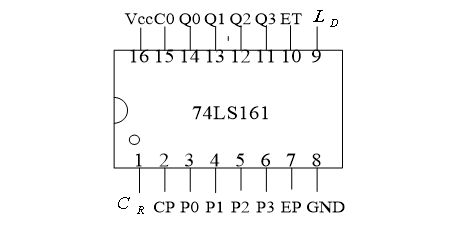
\includegraphics[width=3.5in]{H:/电子技术试验/4-21/4-21-1.png}
        \caption{74LS161引脚图} \label{fig:aa}
        \end{figure}
       
       
        \begin{figure}[h]
            %\small
            \centering
            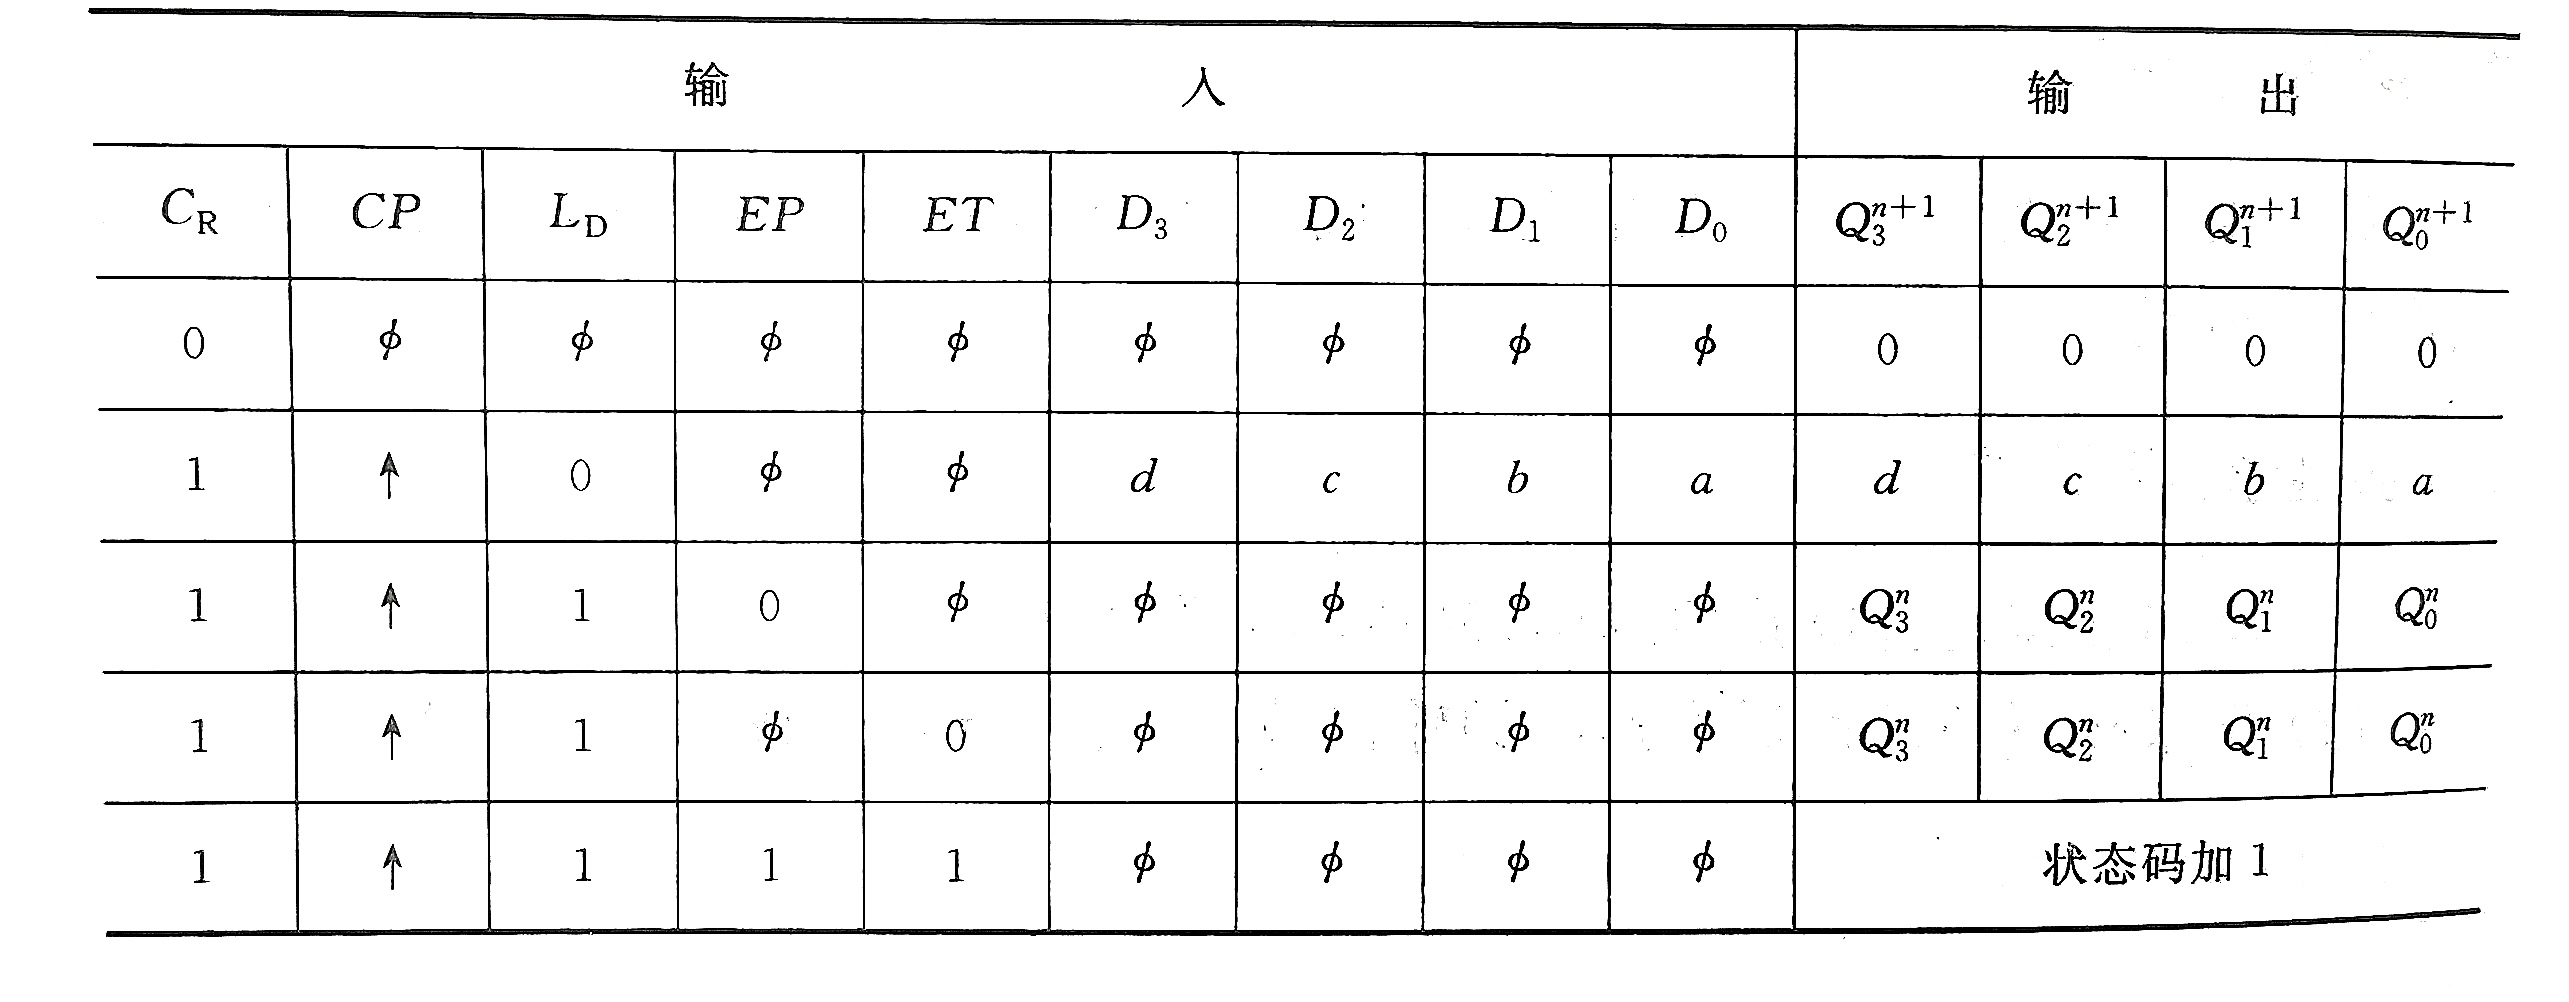
\includegraphics[width=3.5in]{H:/电子技术试验/4-21/4-21-2.jpg}
            \caption{74LS161真值表} \label{fig:aa}
            \end{figure}

            从功能表中可知,当清零端$ C_R="0"$时,计数器输出$Q_1,Q_2,Q_3,Q_0$。立即为全"0",这是异步复位功能。当$ C_R="1"$且$L_D="0"$时,
            在.CP 脉冲上升沿作用后,74LS161的输出端$Q_1,Q_2,Q_3,Q_0$,的状态分别与并行数据输入端 D3,D2,D1,D0的状态相同,
            这是同步置数功能。而当$ C_R=L_D="1"$、EP与 ET中有一个为"0"时,计数器不计数,输出端状态保持不变。只有当$ C_R=L_D=EP=ET="1"$时,
            CP 脉冲上升沿作用后,计数 器 加1。此 外,74LS161 还 有一个 进 位 输 出 端 C。,其 逻 辑关 系是 $ C_0=Q_3Q_2Q_1Q_0ET$。\par
            合理应用计数器的清零功能和置数功能,一片74LS161可以构成分频数16 以下的任意进制分频器。\par 
            (1)用异步清零功能设计分频数为 16 以下的任意进制分频器\par 
            图 2 是9 分频器的电路原理图。图中每个 CP脉冲作用后,74LS161 就加"1",当$Q_0=Q_1=Q_2="1"$时,
            四输入与非门74LS20输入全"1"、输出为"0"。计数器立即复位并重新开始计数。74LS161输出端随时钟脉冲输入的变化规律列于表 2。
            每输入9个时钟脉冲,复位控制与非门的输出端就有一个很窄的负脉冲,脉冲的宽度约为 2t,时间。同理可得图3,
            表示不同分频数时复位控制与非门输入端和74LS161 输出端的连接规律,四输入与非门的多余输入端接高电平。
            异步复位时在计数器输出端上可能会出现不应有的毛刺信号。
            \begin{figure}[h]
                %\small
                \centering
                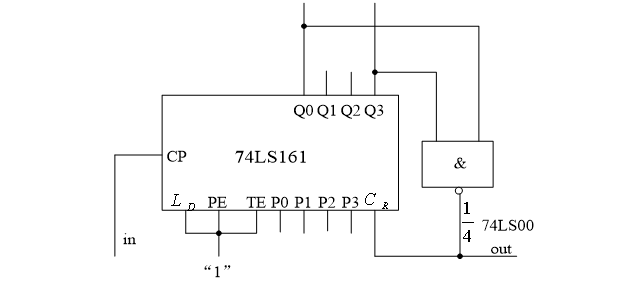
\includegraphics[width=3.5in]{H:/电子技术试验/4-21/4-21-3.png}
                \caption{9分频器的电路原理图} \label{fig:aa}
                \end{figure}
    

            \begin{table}[h]
                \centering  
                \begin{tabular}{c|c|c|c|c}
                    \hline
                          CP             & $Q_3$  &$Q_2$  &$Q_1$  &$Q_0$  \\ \hline
                          0              & 0      &0      & 0     & 0     \\ \hline
                          1              & 0      &0      & 0     & 1            \\ \hline
                          2              & 0      &0      & 1     & 0            \\ \hline
                          3              & 0      &0      & 1     & 1            \\ \hline
                          4              & 0      &1      & 0     & 0            \\ \hline
                          5              & 0      &1      & 0     & 1           \\ \hline
                          6              & 0      &1      & 1     & 0           \\ \hline
                          7              & 0      &1      & 1     & 1           \\ \hline
                          8              & 1      &0      & 0     & 0           \\ \hline
                          9              & 0      &0      & 0     & 0           \\ \hline
                        \end{tabular}
              \end{table}
  \begin{figure}[h]
    %\small
    \centering
    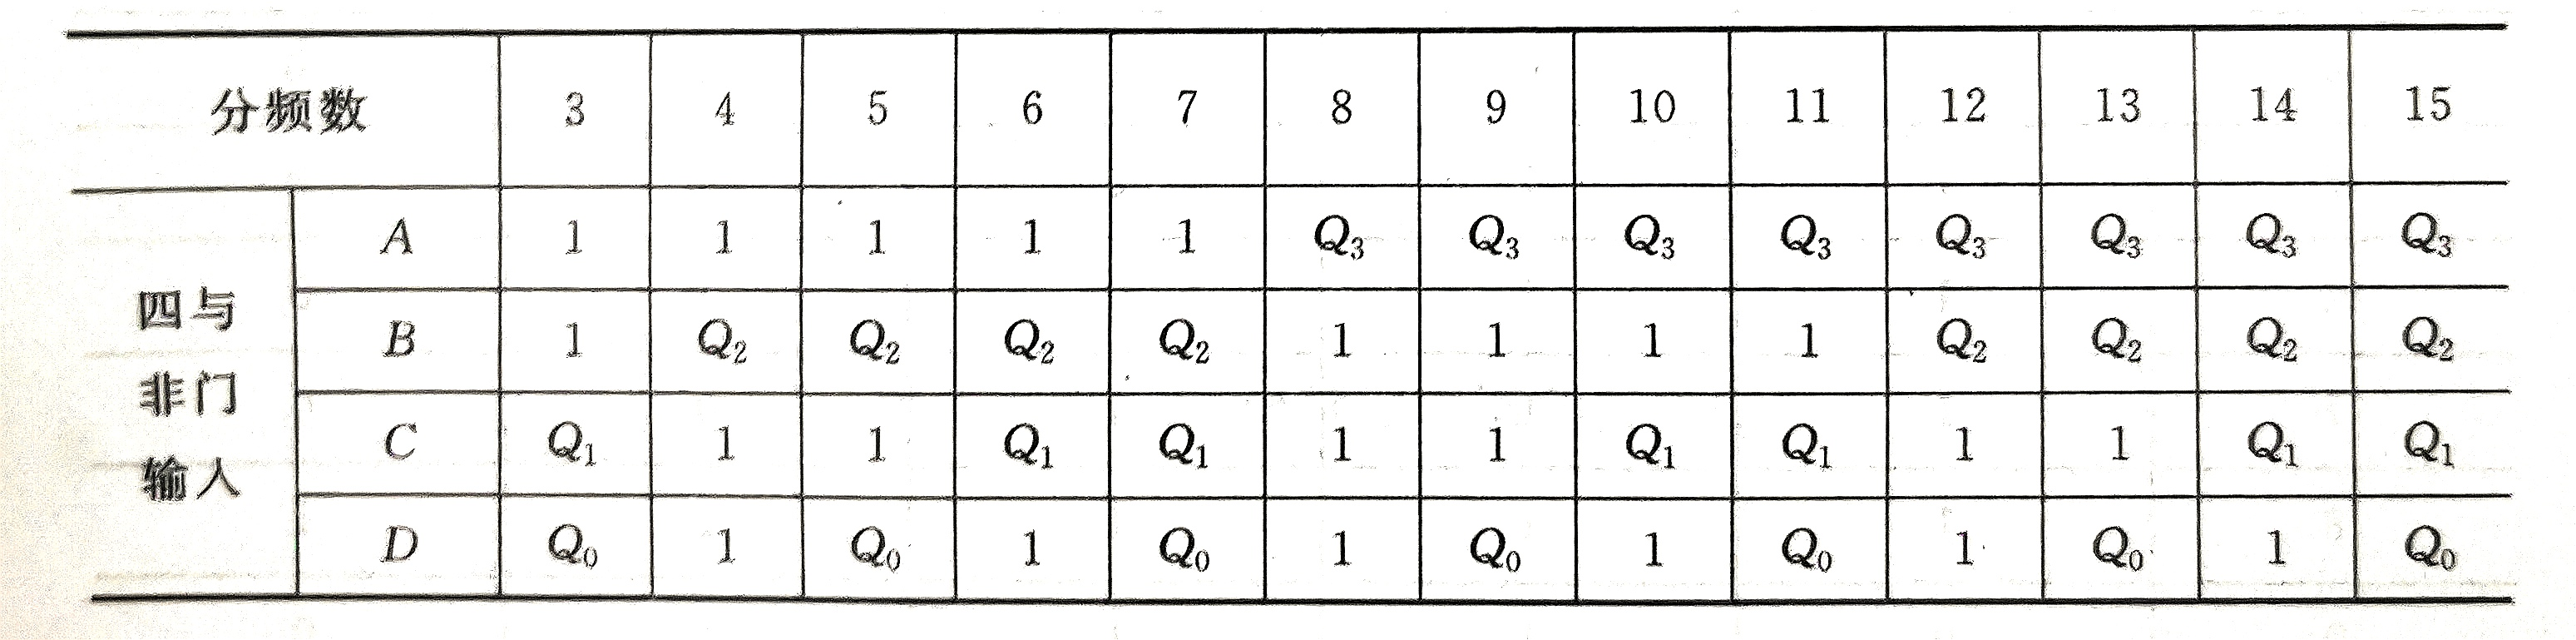
\includegraphics[width=3.5in]{H:/电子技术试验/4-21/4-21-4.jpg}
    \caption{与非门输入端与分频数关系表} \label{fig:aa}
    \end{figure}
\par

    (2)利用同步置数法实现分频数为 16 以下的任意进制分频\par
    图 4 是由74LS161和反相器组成的12分频器,利用进位信号 C0反相后产生预置数控制信号。在CP脉冲作用后,74LS161 就加1。
    当Q3=Q2=Q1=Q0=ET="1"时,进位端C0,输出为"1",反相后使74LS161的置位控制端LD有效,计数器进入置数准备状态。当下一个时钟脉冲上升沿到达时,
    数据输入端 D3,D2,D1,D0的数据被置入内部触发器,完成置数功能。LD端的脉冲频率为计数时钟的12分频,负脉冲宽度为一个时钟周期。
    利用进位信号 C0同步置数的电路分频数 N 为
  \[  N=D3'×2^3+D2'×2^2+D1'×2^1+D0'×2^0+1 \]
    式中,D3,D2,D1,D0。接地时为"0",否则为"1"。例如,图 4-4-3中,D3="0",D2=D1=D0="1",代入式 1中可得分频数为
    \[  N=1'×2^3+0'×2^2+1'×2^1+1'×2^0+1=12 \]

    \begin{figure}[h]
        %\small
        \centering
        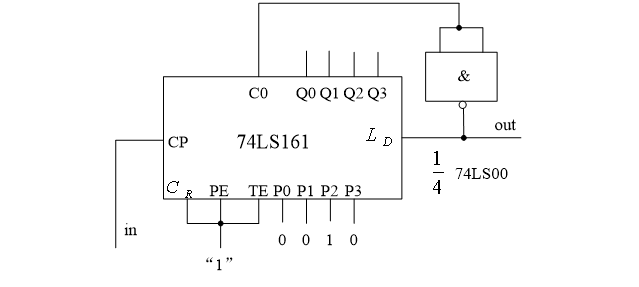
\includegraphics[width=3.5in]{H:/电子技术试验/4-21/4-21-5.png}
        \caption{12分频器的电路原理图} \label{fig:aa}
        \end{figure}


        表2列出了图5电路在每个时钟脉冲CP作用下Q1,Q2,Q3,Q0和 C0的输出的状态。\par
        \begin{table}[h]
            \centering  
            \begin{tabular}{c|c|c|c|c|c}
                \hline
                      CP             & $Q_3$  &$Q_2$  &$Q_1$  &$Q_0$  &$C_0$      \\ \hline
                      0              & 0      &1      & 0     & 0     &0 \\ \hline
                      1              & 0      &1      & 0     & 1     &0 \\ \hline
                      2              & 0      &1      & 1     & 0     &0 \\ \hline
                      3              & 0      &1      & 1     & 1     &0 \\ \hline
                      4              & 1      &0      & 0     & 0     &0 \\ \hline
                      5              & 1      &0      & 0     & 1     &0 \\ \hline
                      6              & 1      &0      & 1     & 0     &0 \\ \hline
                      7              & 1      &0      & 1     & 1     &0 \\ \hline
                      8              & 1      &1      & 0     & 0     &0 \\ \hline
                      9              & 1      &1      & 0     & 1     &0 \\ \hline
                      10             & 1      &1      & 1     & 0     &0 \\ \hline
                      11             & 1      &1      & 1     & 1     &1 \\ \hline
                      12             & 0      &1      & 0     & 0     &0 \\ \hline
                    \end{tabular}
          \end{table}

    \par
    
\newpage
\section{\zihao{4} 实验电路}
\begin{figure}[h]
    %\small
    \centering
    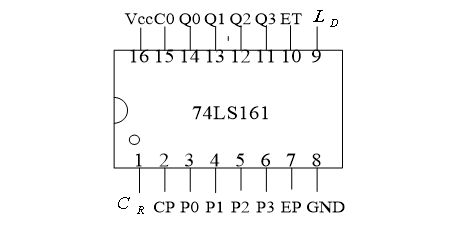
\includegraphics[width=3.5in]{H:/电子技术试验/4-21/4-21-1.png}
    \caption{74LS161引脚图} \label{fig:aa}
    \end{figure}
   
\begin{figure}[h]
    %\small
    \centering
    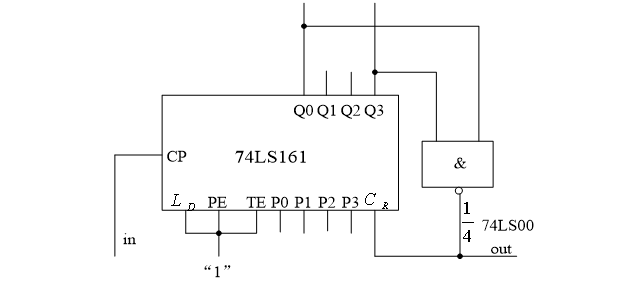
\includegraphics[width=3.5in]{H:/电子技术试验/4-21/4-21-3.png}
    \caption{9分频器的电路原理图} \label{fig:aa}
    \end{figure}


    \begin{figure}[h]
        %\small
        \centering
        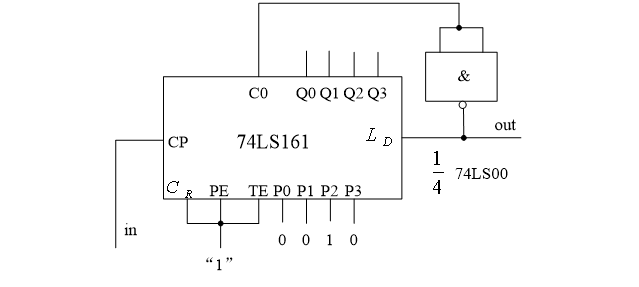
\includegraphics[width=3.5in]{H:/电子技术试验/4-21/4-21-5.png}
        \caption{12分频器的电路原理图} \label{fig:aa}
        \end{figure}

\newpage

\section{\zihao{4} 实验内容及步骤}
1.按图4-4-1,表4-4-1验证74LS161的功能。\par
2.利用74LS161的清零端CR设计一个9分频器。当时钟频率为1Hz时,用LED数码管显示74LS161 Q3—Q0的输出状态,
并填入表3中。当时钟频率为10kHz时,用示波器观察和记录CP,Q3—Q0的波形。\par
3. 利用74LS161的置数端LD设计一个12分频器。当时钟频率为1Hz时,用LED显示74LS161 Q3—Q0的输出状态,并填入表4中。
当时钟频率为10kHz时,用示波器观察和记录CP,CO,Q3—Q0的波形。\par



\section{\zihao{4} 实验设备和器材}
(1)直流稳压电源             \qquad \quad \qquad \qquad \qquad \qquad           1台\par
(2)数字逻辑实验箱            \qquad  \qquad \qquad \qquad\qquad                1台\par
(3)74LS00、74LS161 \qquad    \quad                                    2片\par
(4)示波器 \qquad  \qquad \qquad \qquad\qquad  \qquad  \qquad    1台\par
 (5)导线   
\section{\zihao{4} 数据及误差处理}
(1)9分频器\par
Q3—Q0的输出状态:  \par
1Hz:\par
% paragraph  (end)
\begin{table}[h]
  \centering  
  \begin{tabular}{c|c|c|c|c}
      \hline
            CP             & $Q_3$  &$Q_2$  &$Q_1$  &$Q_0$  \\ \hline
            0              & 0      &0      & 0     & 0     \\ \hline
            1              & 0      &0      & 0     & 1            \\ \hline
            2              & 0      &0      & 1     & 0            \\ \hline
            3              & 0      &0      & 1     & 1            \\ \hline
            4              & 0      &1      & 0     & 0            \\ \hline
            5              & 0      &1      & 0     & 1           \\ \hline
            6              & 0      &1      & 1     & 0           \\ \hline
            7              & 0      &1      & 1     & 1           \\ \hline
            8              & 1      &0      & 0     & 0           \\ \hline
            9              & 0      &0      & 0     & 0           \\ \hline
          \end{tabular}
\end{table}
\par
\newpage
1OkHz:\par
\begin{figure}[h]
  \begin{minipage}[t]{0.5\linewidth} % 如果一行放2个图,用0.5,如果3个图,用0.33  
    \centering   
    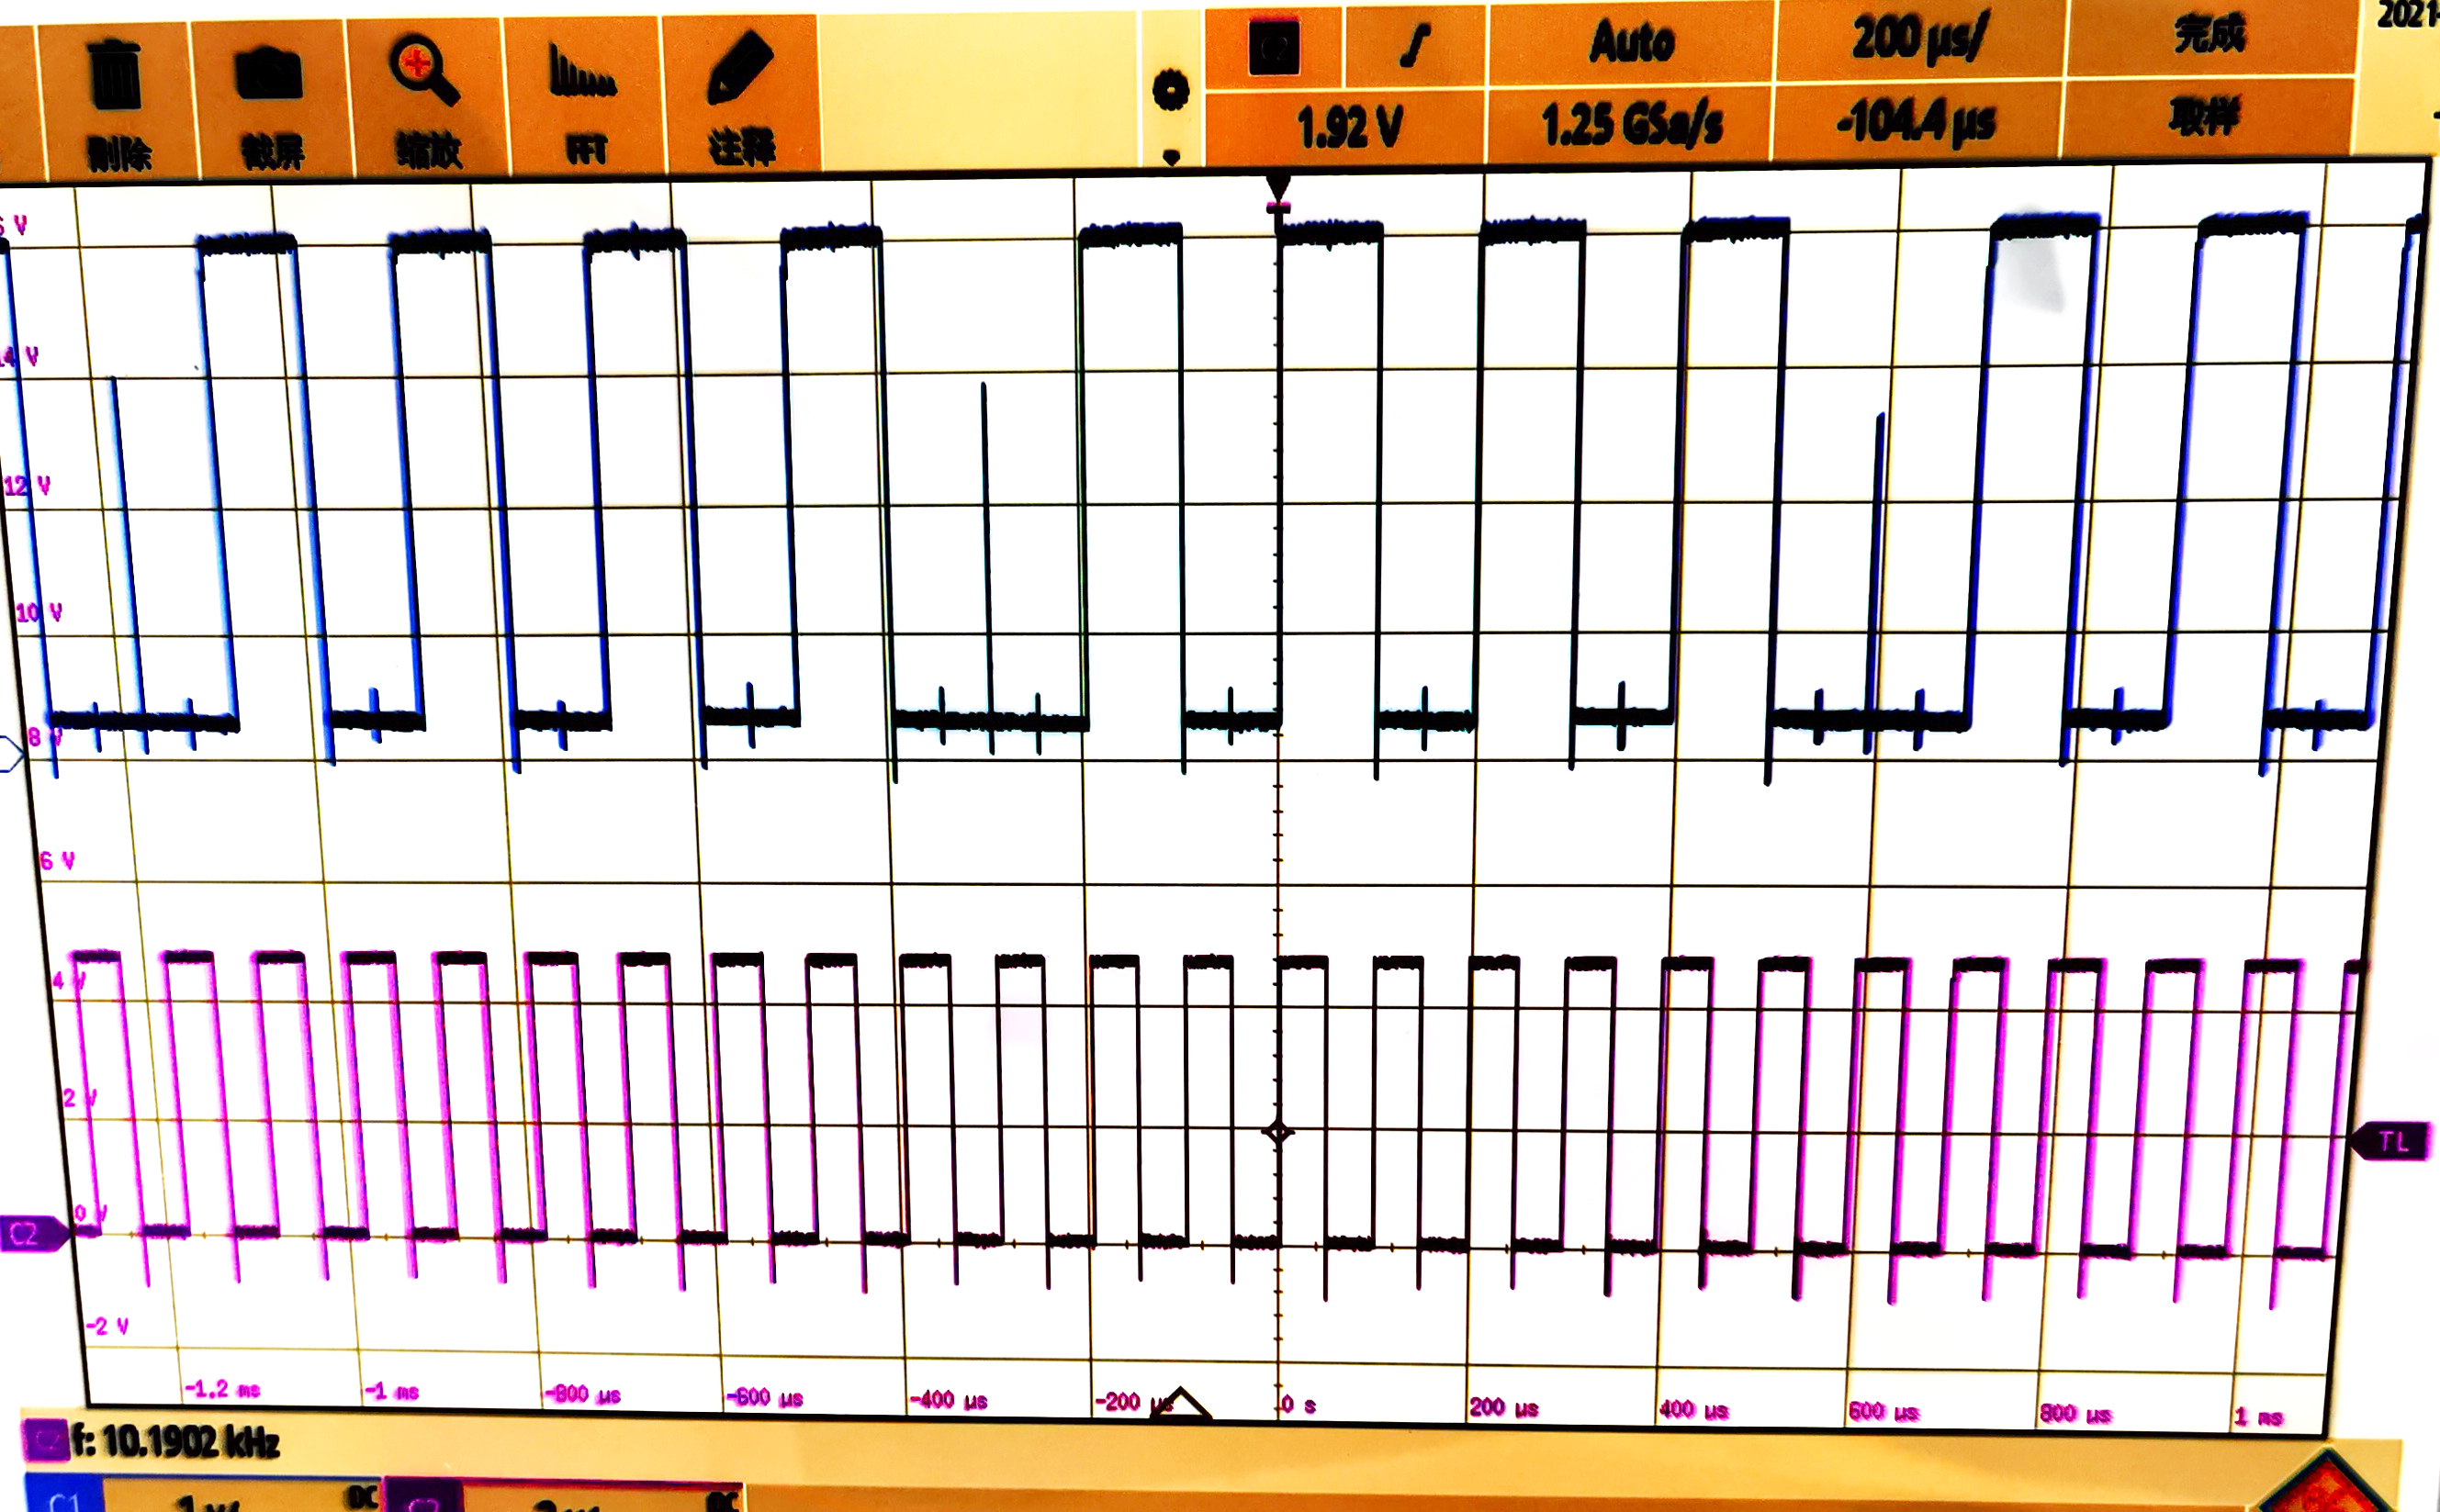
\includegraphics[width=3.5in]{H:/电子技术试验/4-21/9-q0.png}   
    \caption{$CLK/Q0$}   
    \label{fig:side:a}   
  \end{minipage}%   
  \begin{minipage}[t]{0.5\linewidth}   
    \centering   
    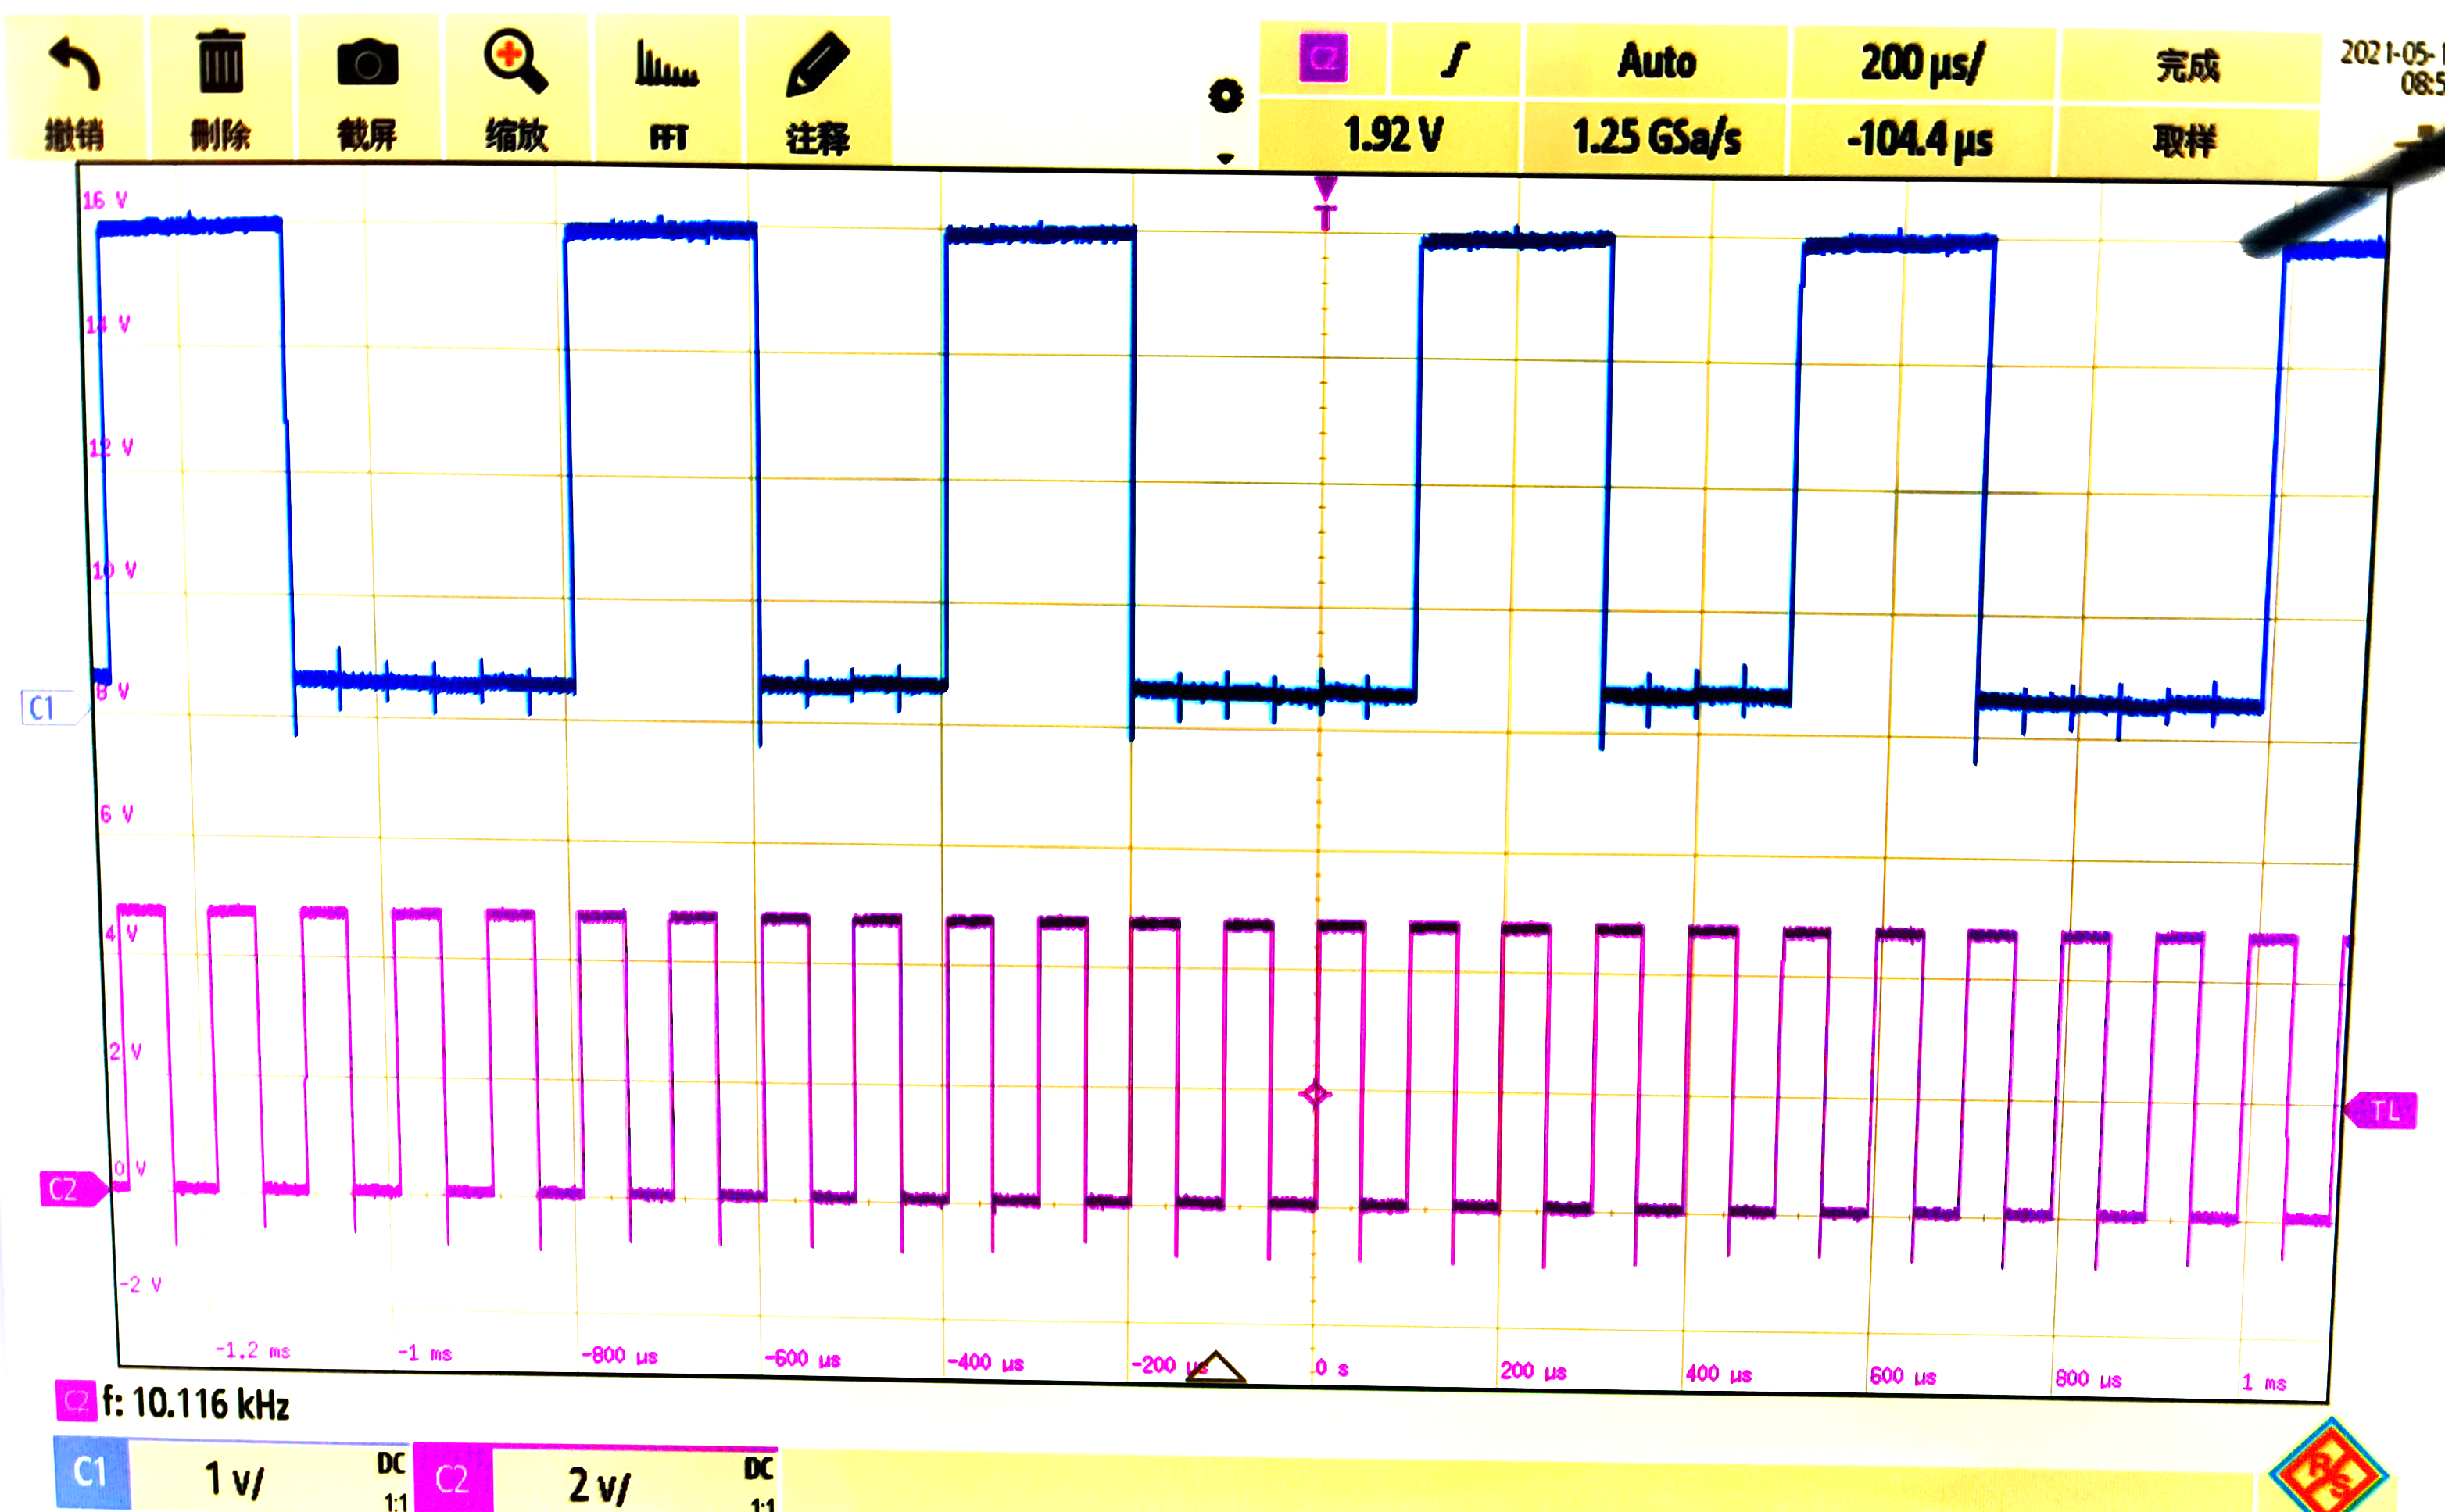
\includegraphics[width=3.5in]{H:/电子技术试验/4-21/9-q1.png}   
    \caption{$CLK/Q1$}   
    \label{fig:side:b}   
  \end{minipage}   
\end{figure}
\begin{figure}[h]
  \begin{minipage}[t]{0.5\linewidth} % 如果一行放2个图,用0.5,如果3个图,用0.33  
    \centering   
    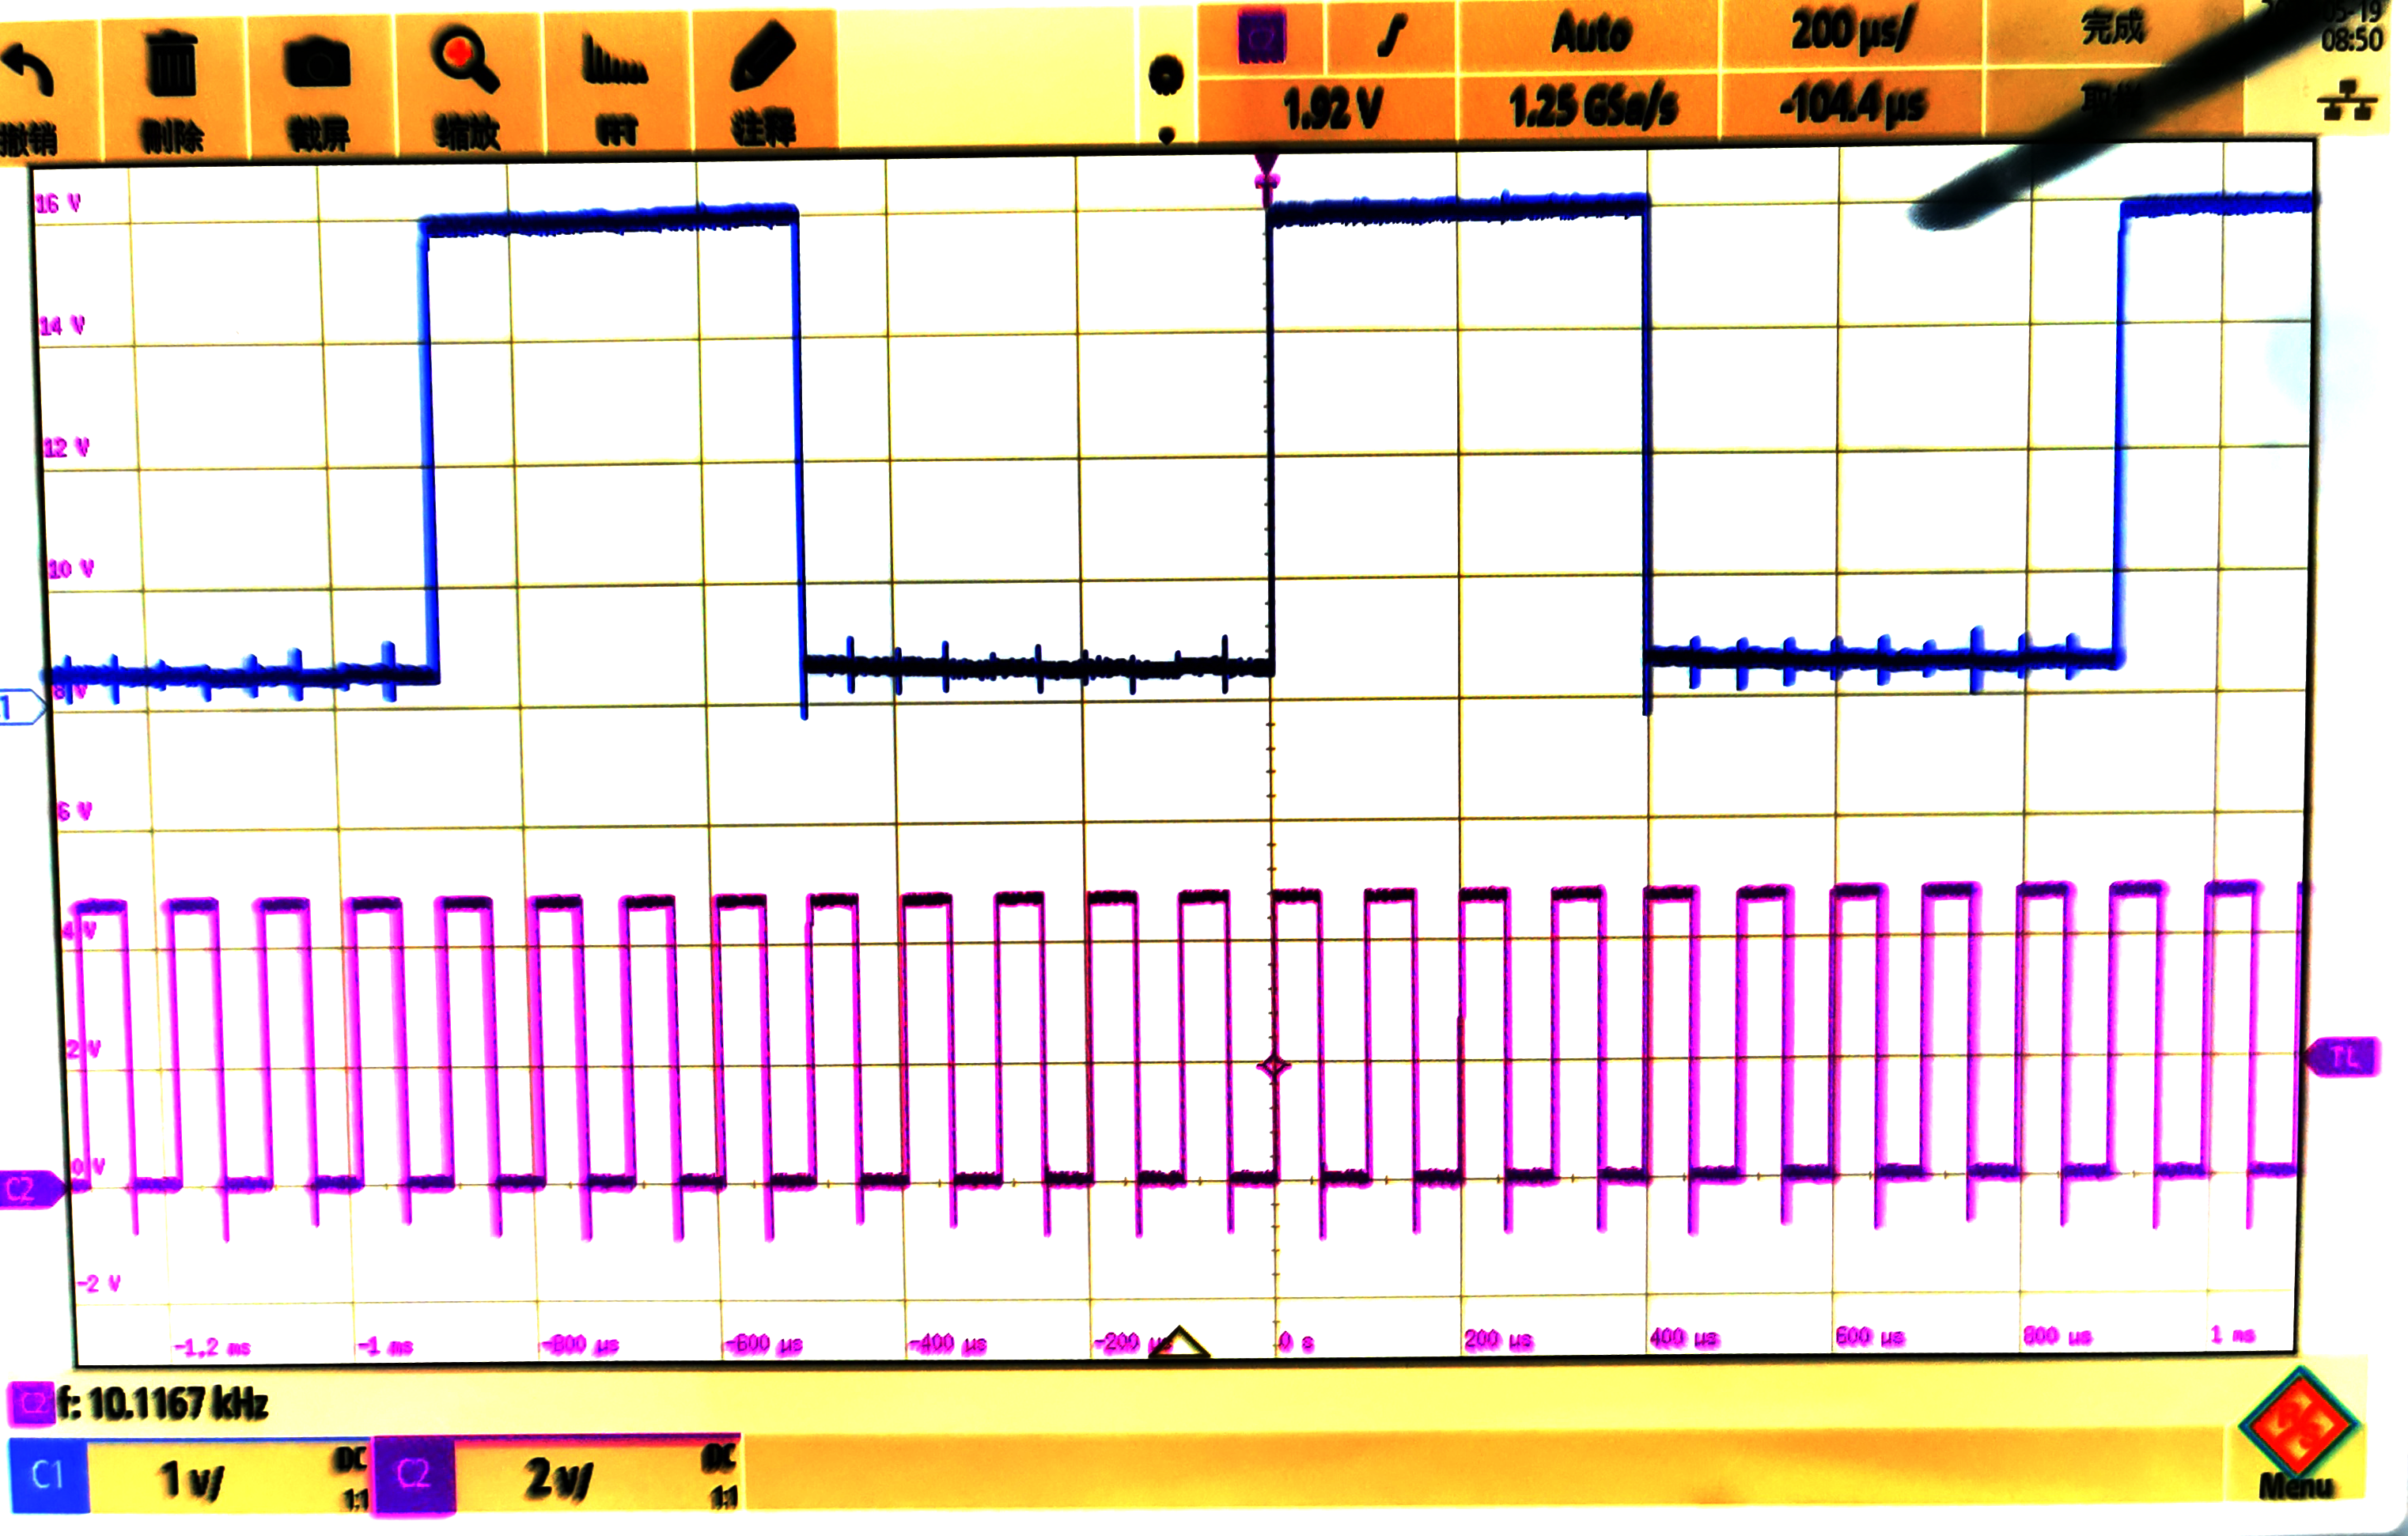
\includegraphics[width=3.5in]{H:/电子技术试验/4-21/9-q2.png}   
    \caption{$CLK/Q2$}   
    \label{fig:side:a}   
  \end{minipage}%   
  \begin{minipage}[t]{0.5\linewidth}   
    \centering   
    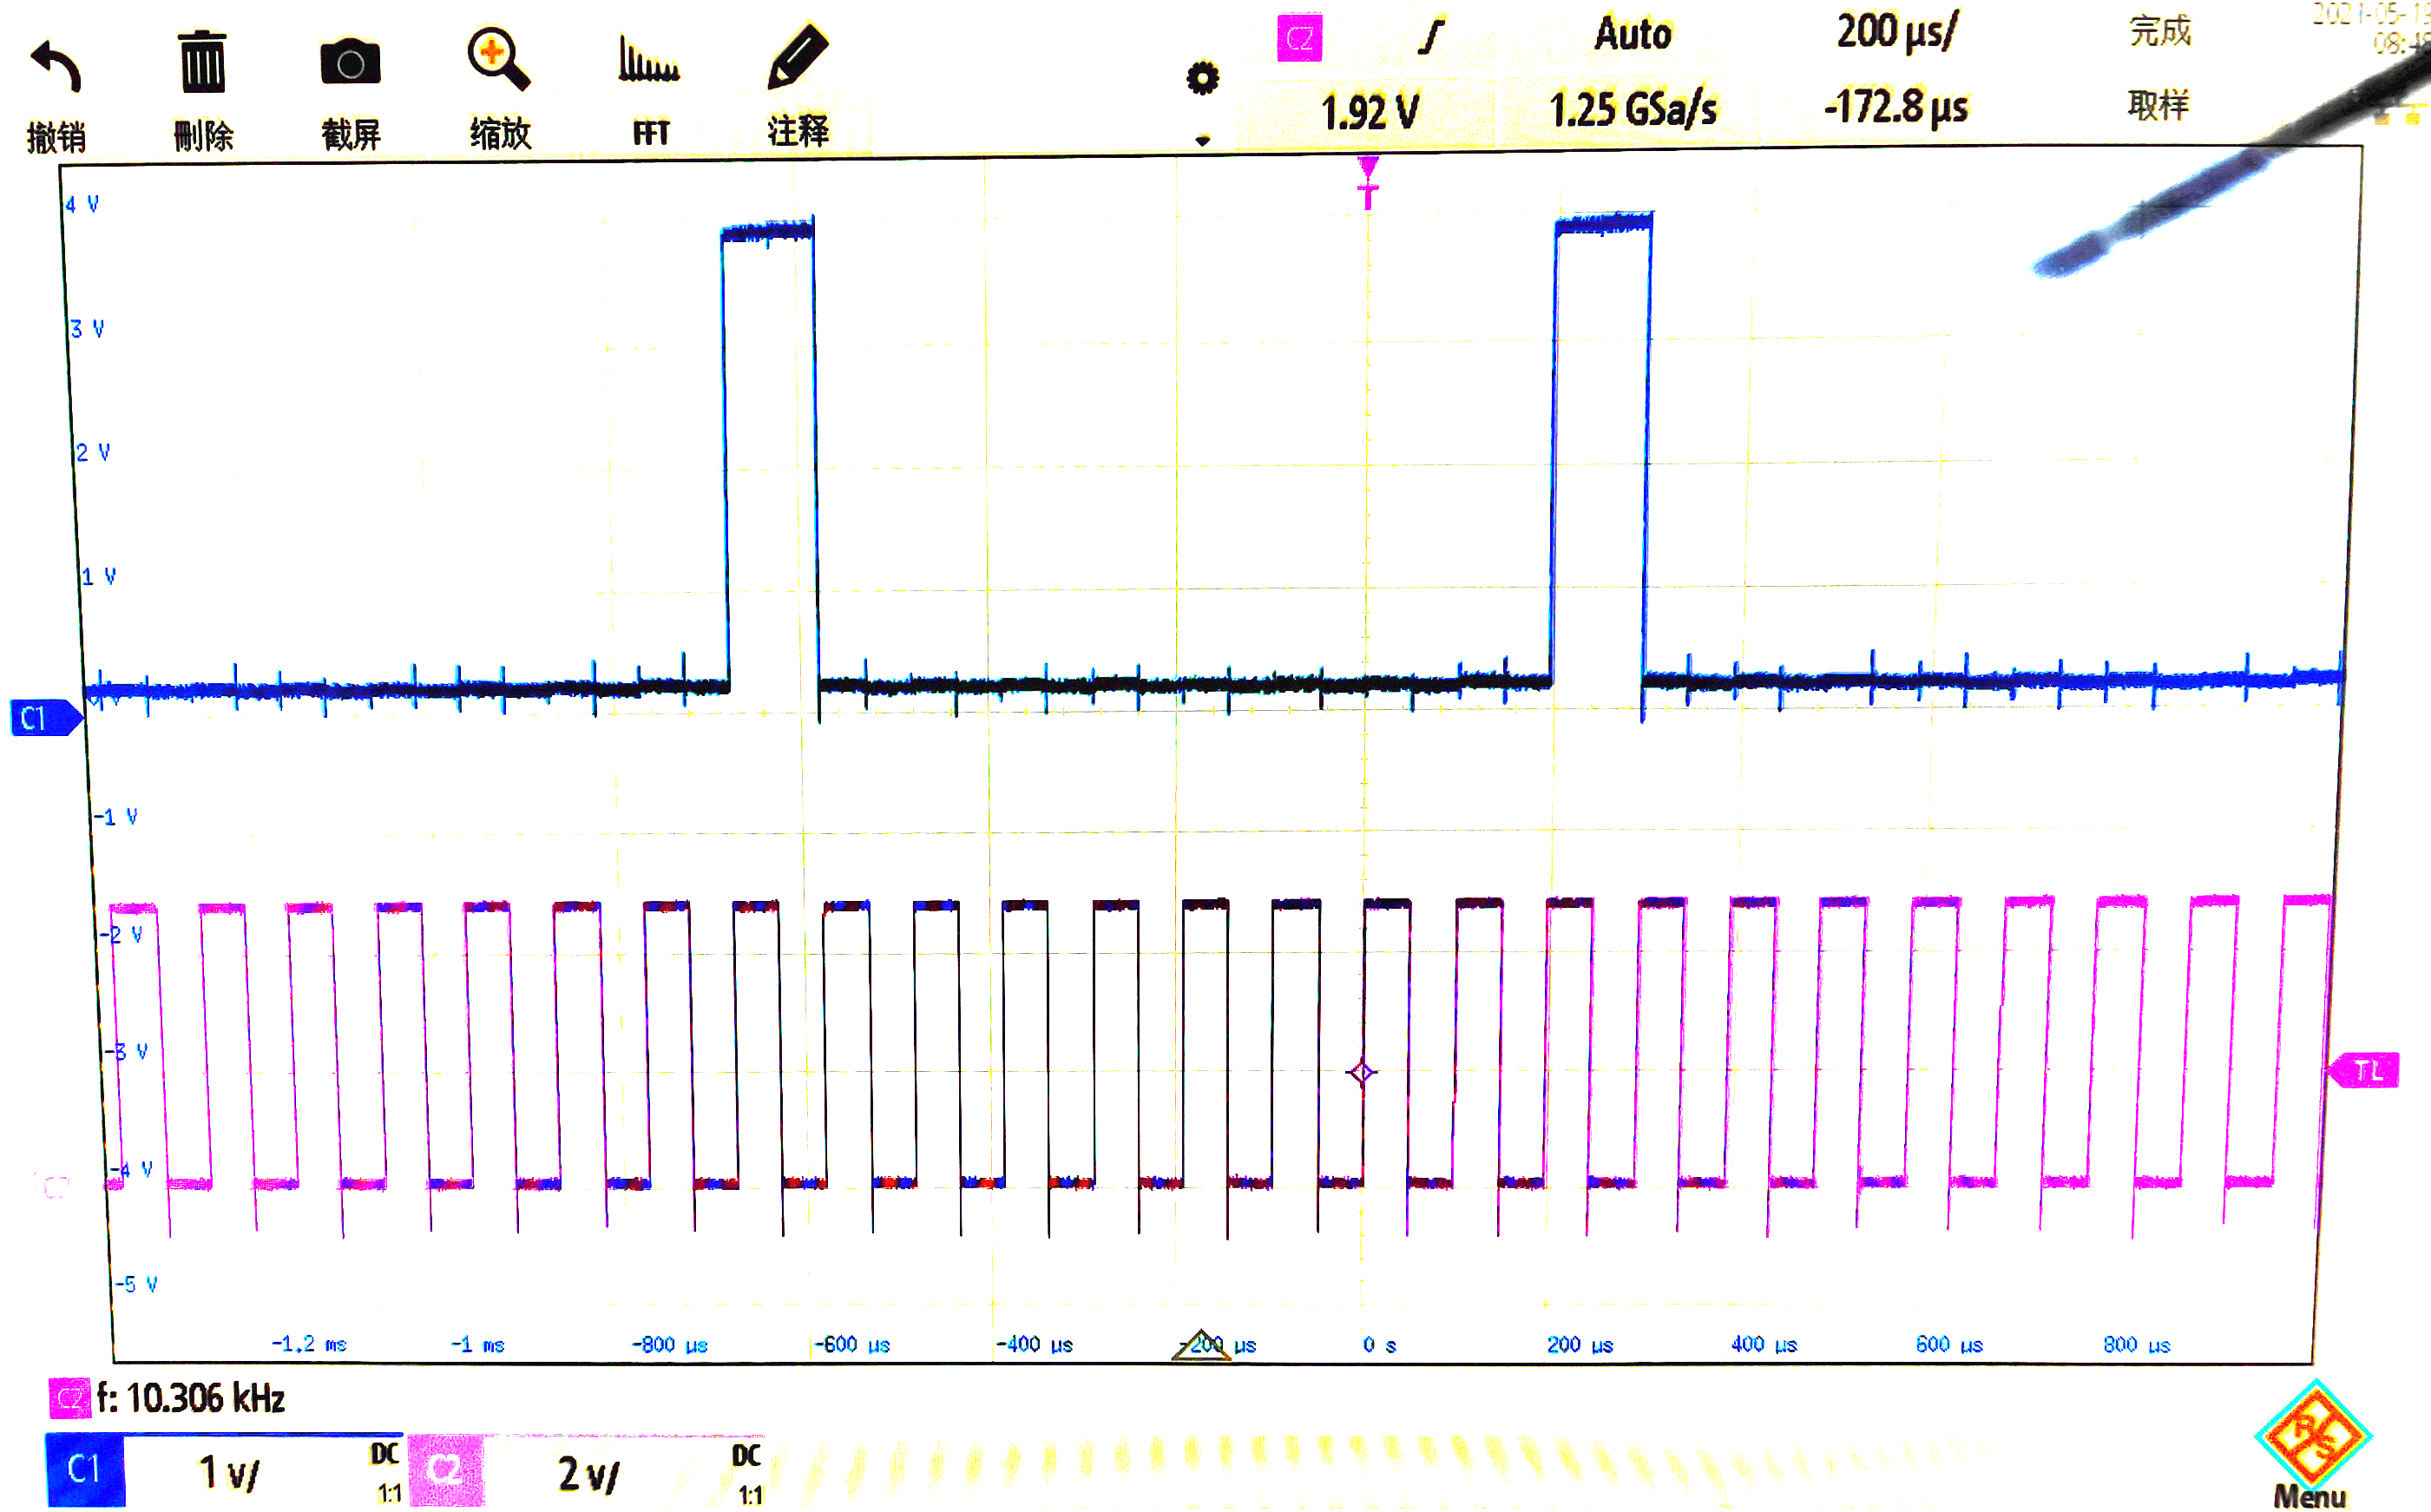
\includegraphics[width=3.5in]{H:/电子技术试验/4-21/9-q3.png}   
    \caption{$CLK/Q3$}   
    \label{fig:side:b}   
  \end{minipage}   
\end{figure}
\par
\newpage
(1)12分频器\par

Q3—Q0的输出状态:  \par
1Hz:\par
\begin{table}[h]
  \centering  
  \begin{tabular}{c|c|c|c|c|c}
      \hline
            CP             & $Q_3$  &$Q_2$  &$Q_1$  &$Q_0$  &$C_0$      \\ \hline
            0              & 0      &1      & 0     & 0     &0 \\ \hline
            1              & 0      &1      & 0     & 1     &0 \\ \hline
            2              & 0      &1      & 1     & 0     &0 \\ \hline
            3              & 0      &1      & 1     & 1     &0 \\ \hline
            4              & 1      &0      & 0     & 0     &0 \\ \hline
            5              & 1      &0      & 0     & 1     &0 \\ \hline
            6              & 1      &0      & 1     & 0     &0 \\ \hline
            7              & 1      &0      & 1     & 1     &0 \\ \hline
            8              & 1      &1      & 0     & 0     &0 \\ \hline
            9              & 1      &1      & 0     & 1     &0 \\ \hline
            10             & 1      &1      & 1     & 0     &0 \\ \hline
            11             & 1      &1      & 1     & 1     &1 \\ \hline
            12             & 0      &1      & 0     & 0     &0 \\ \hline
          \end{tabular}
\end{table}

\par
10kHz:\par
\begin{figure}[h]
  \begin{minipage}[t]{0.5\linewidth} % 如果一行放2个图,用0.5,如果3个图,用0.33  
    \centering   
    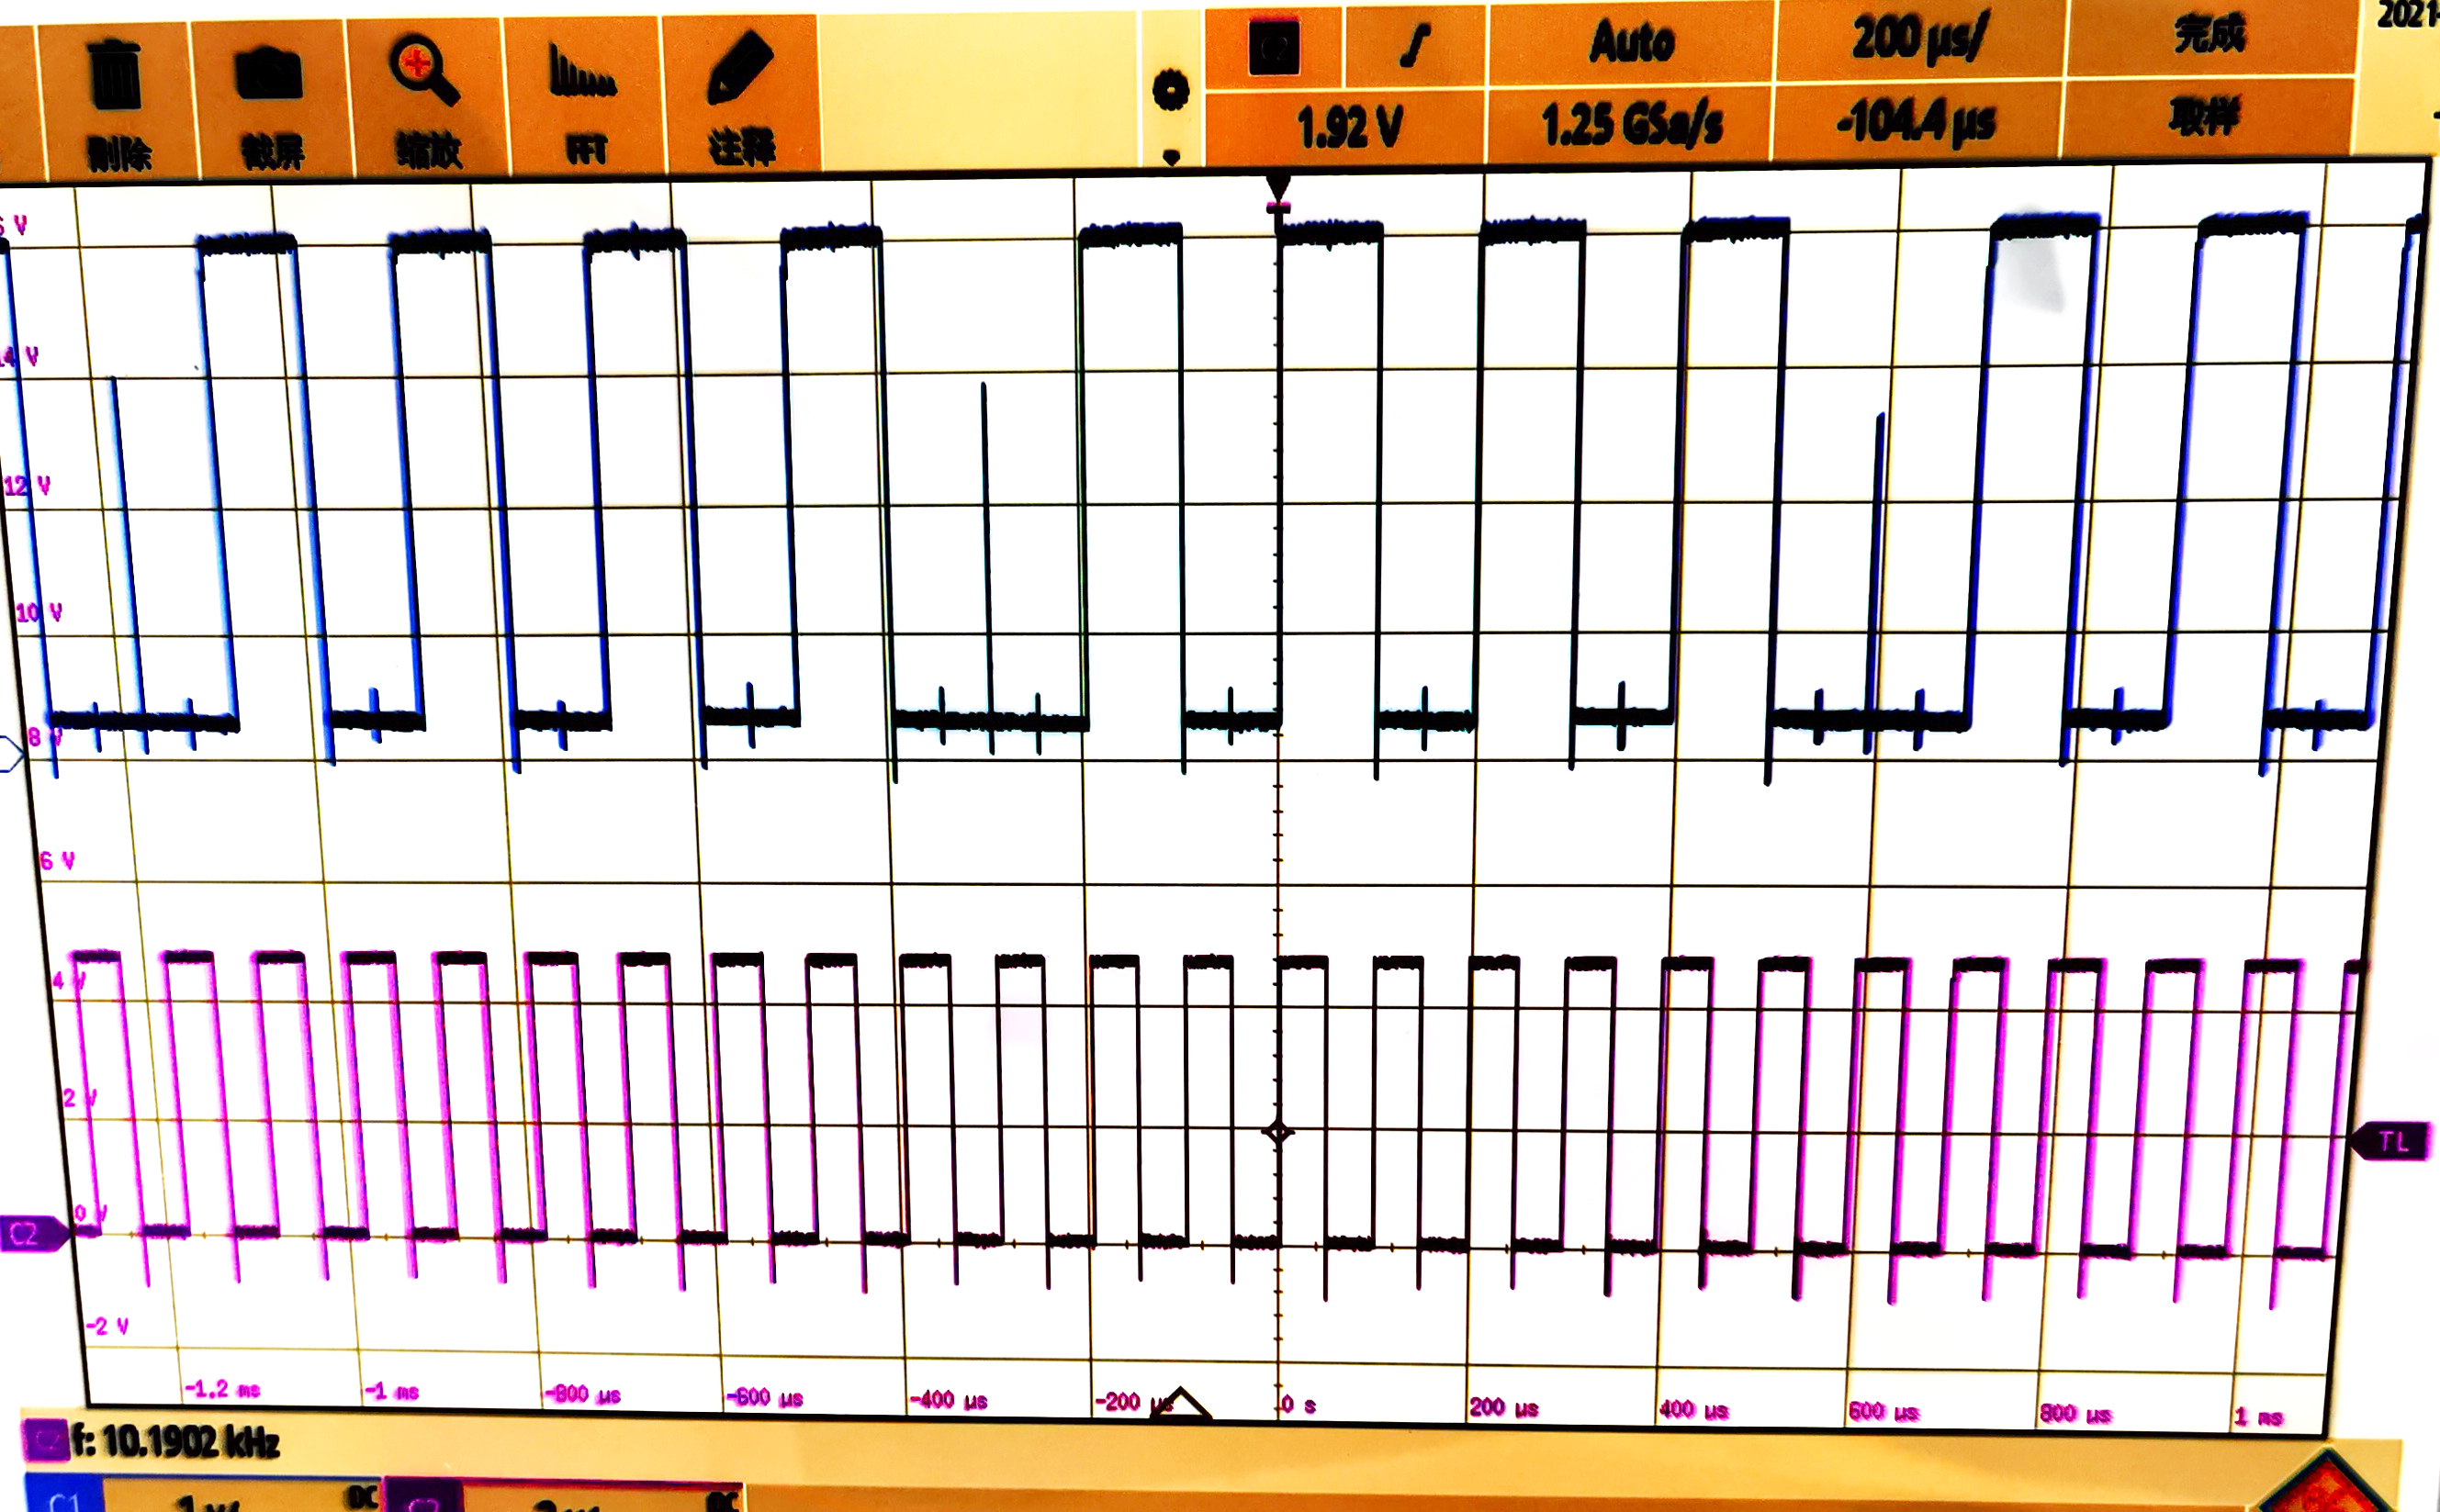
\includegraphics[width=3.5in]{H:/电子技术试验/4-21/9-q0.png}   
    \caption{$CLK/Q0$}   
    \label{fig:side:a}   
  \end{minipage}%   
  \begin{minipage}[t]{0.5\linewidth}   
    \centering   
    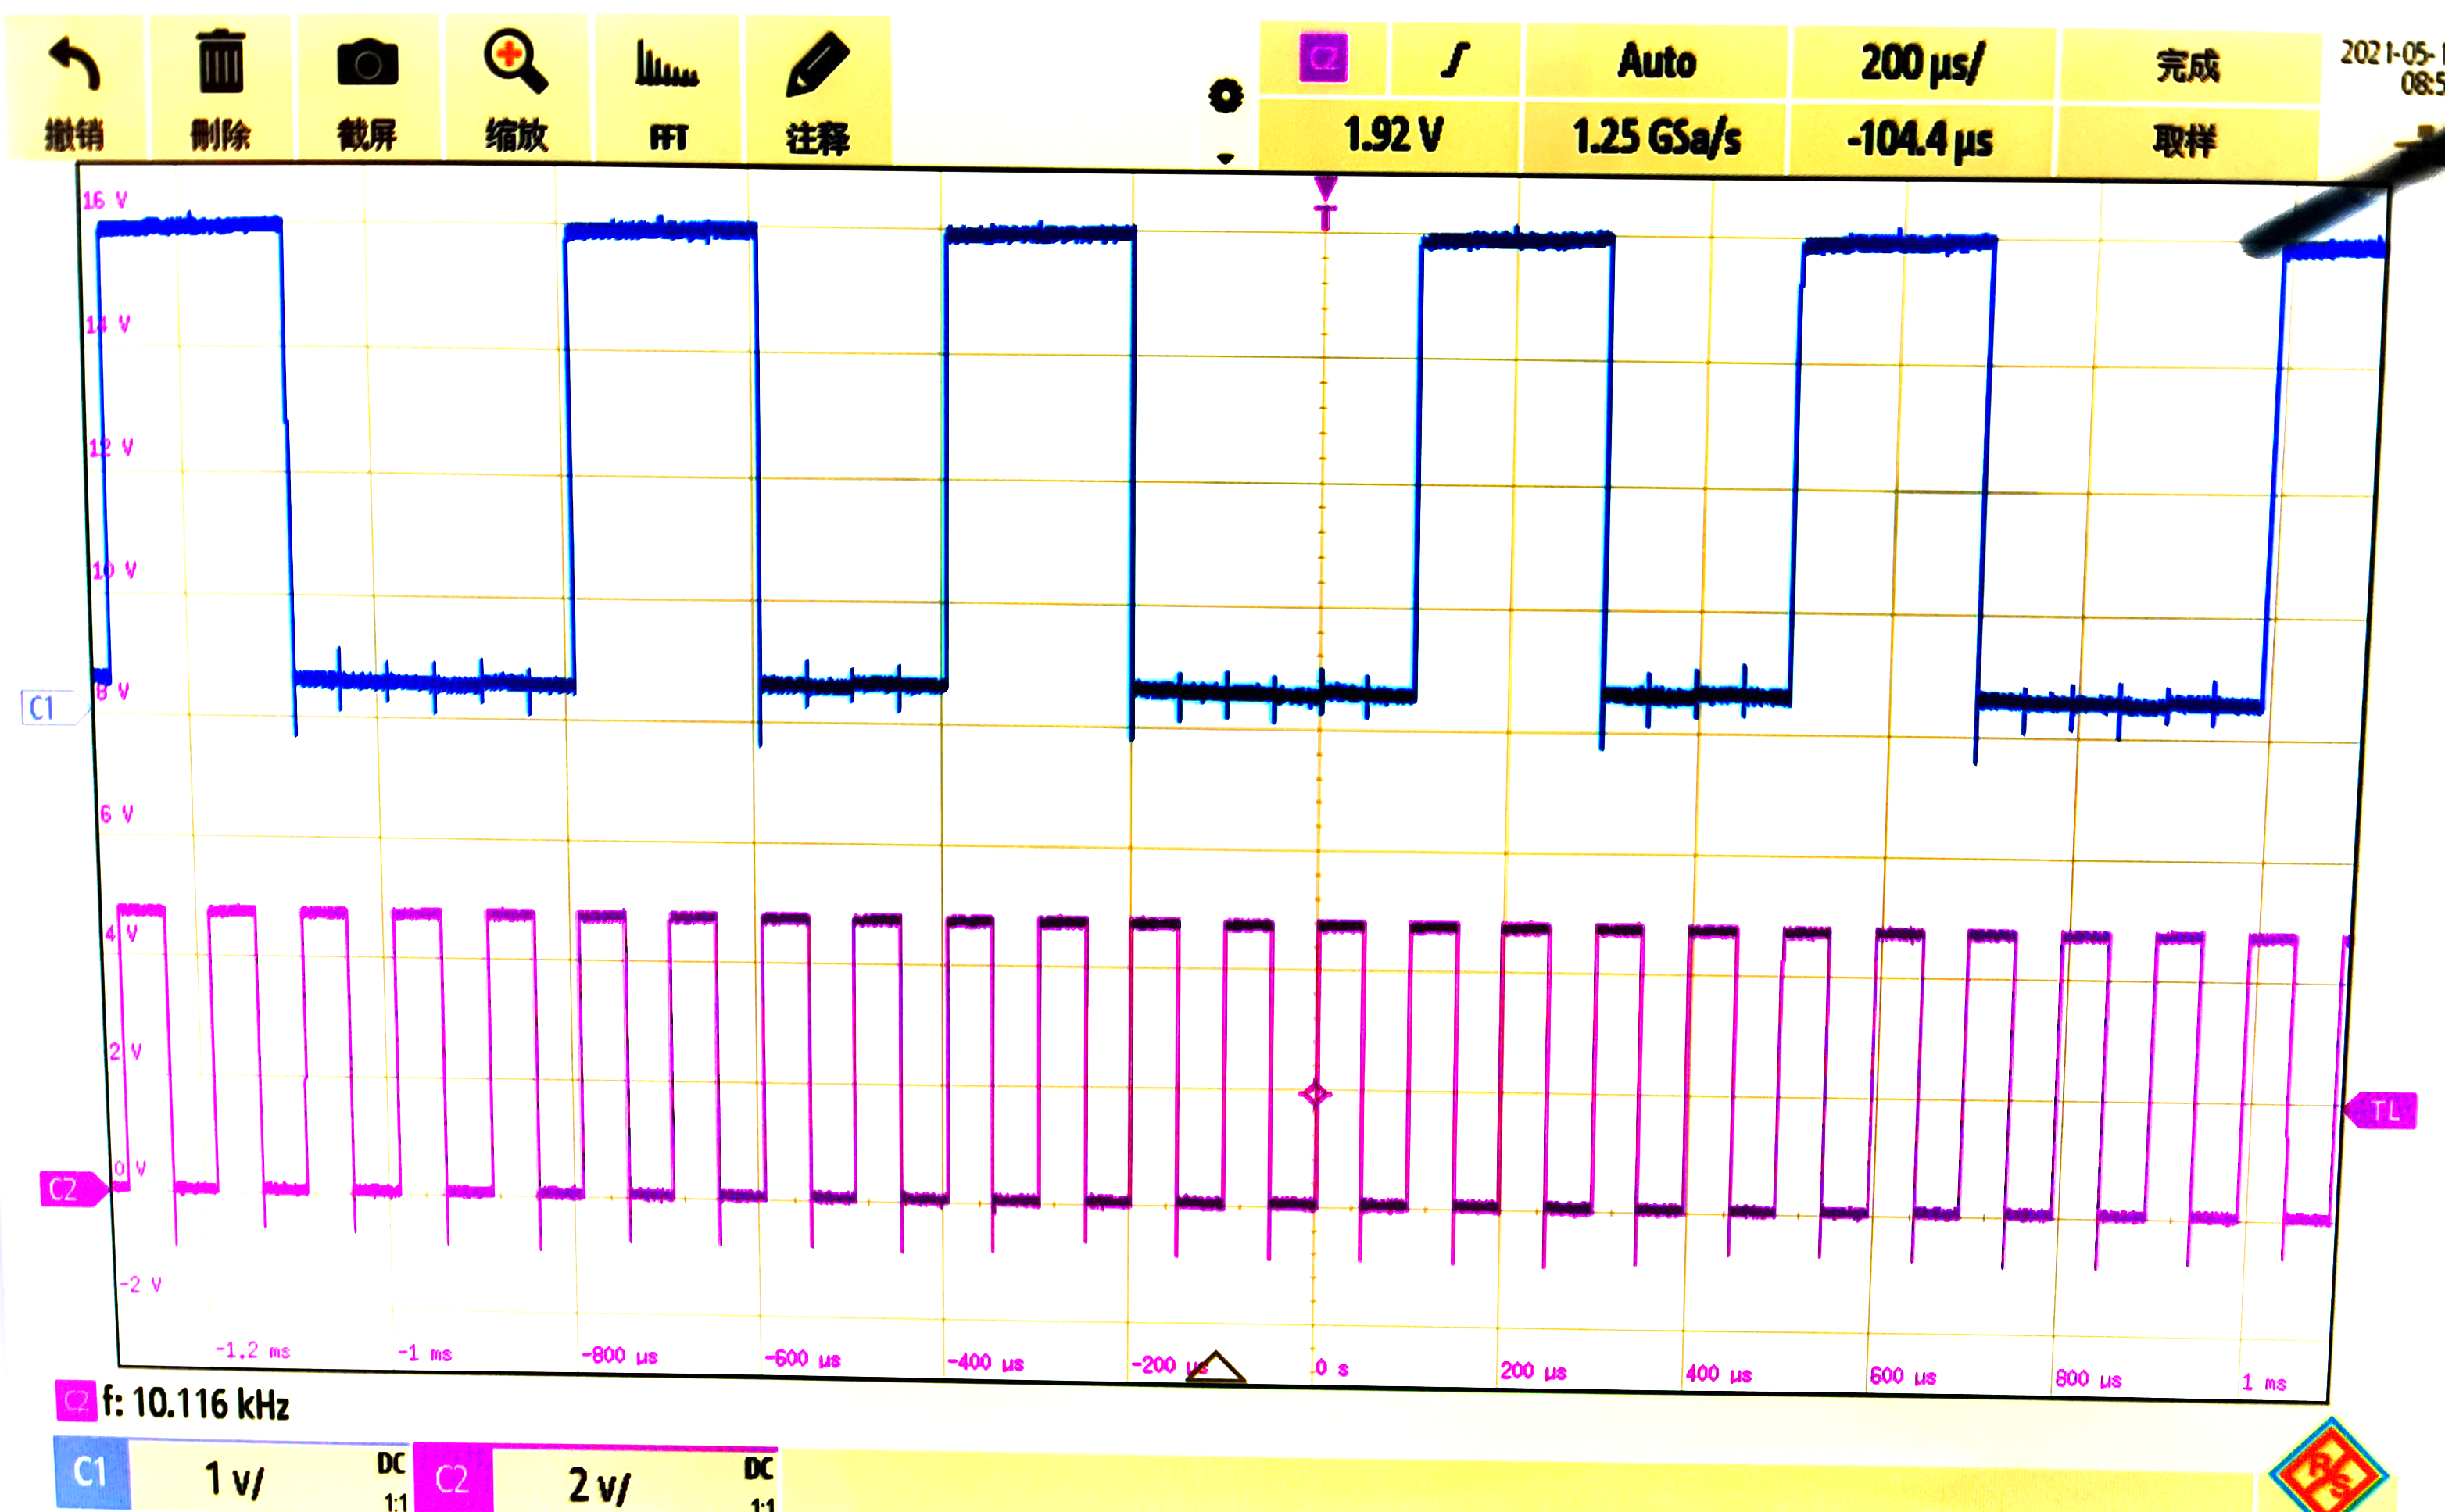
\includegraphics[width=3.5in]{H:/电子技术试验/4-21/9-q1.png}   
    \caption{$CLK/Q1$}   
    \label{fig:side:b}   
  \end{minipage}   
\end{figure}
\newpage
\begin{figure}[h]
  \begin{minipage}[t]{0.5\linewidth} % 如果一行放2个图,用0.5,如果3个图,用0.33  
    \centering   
    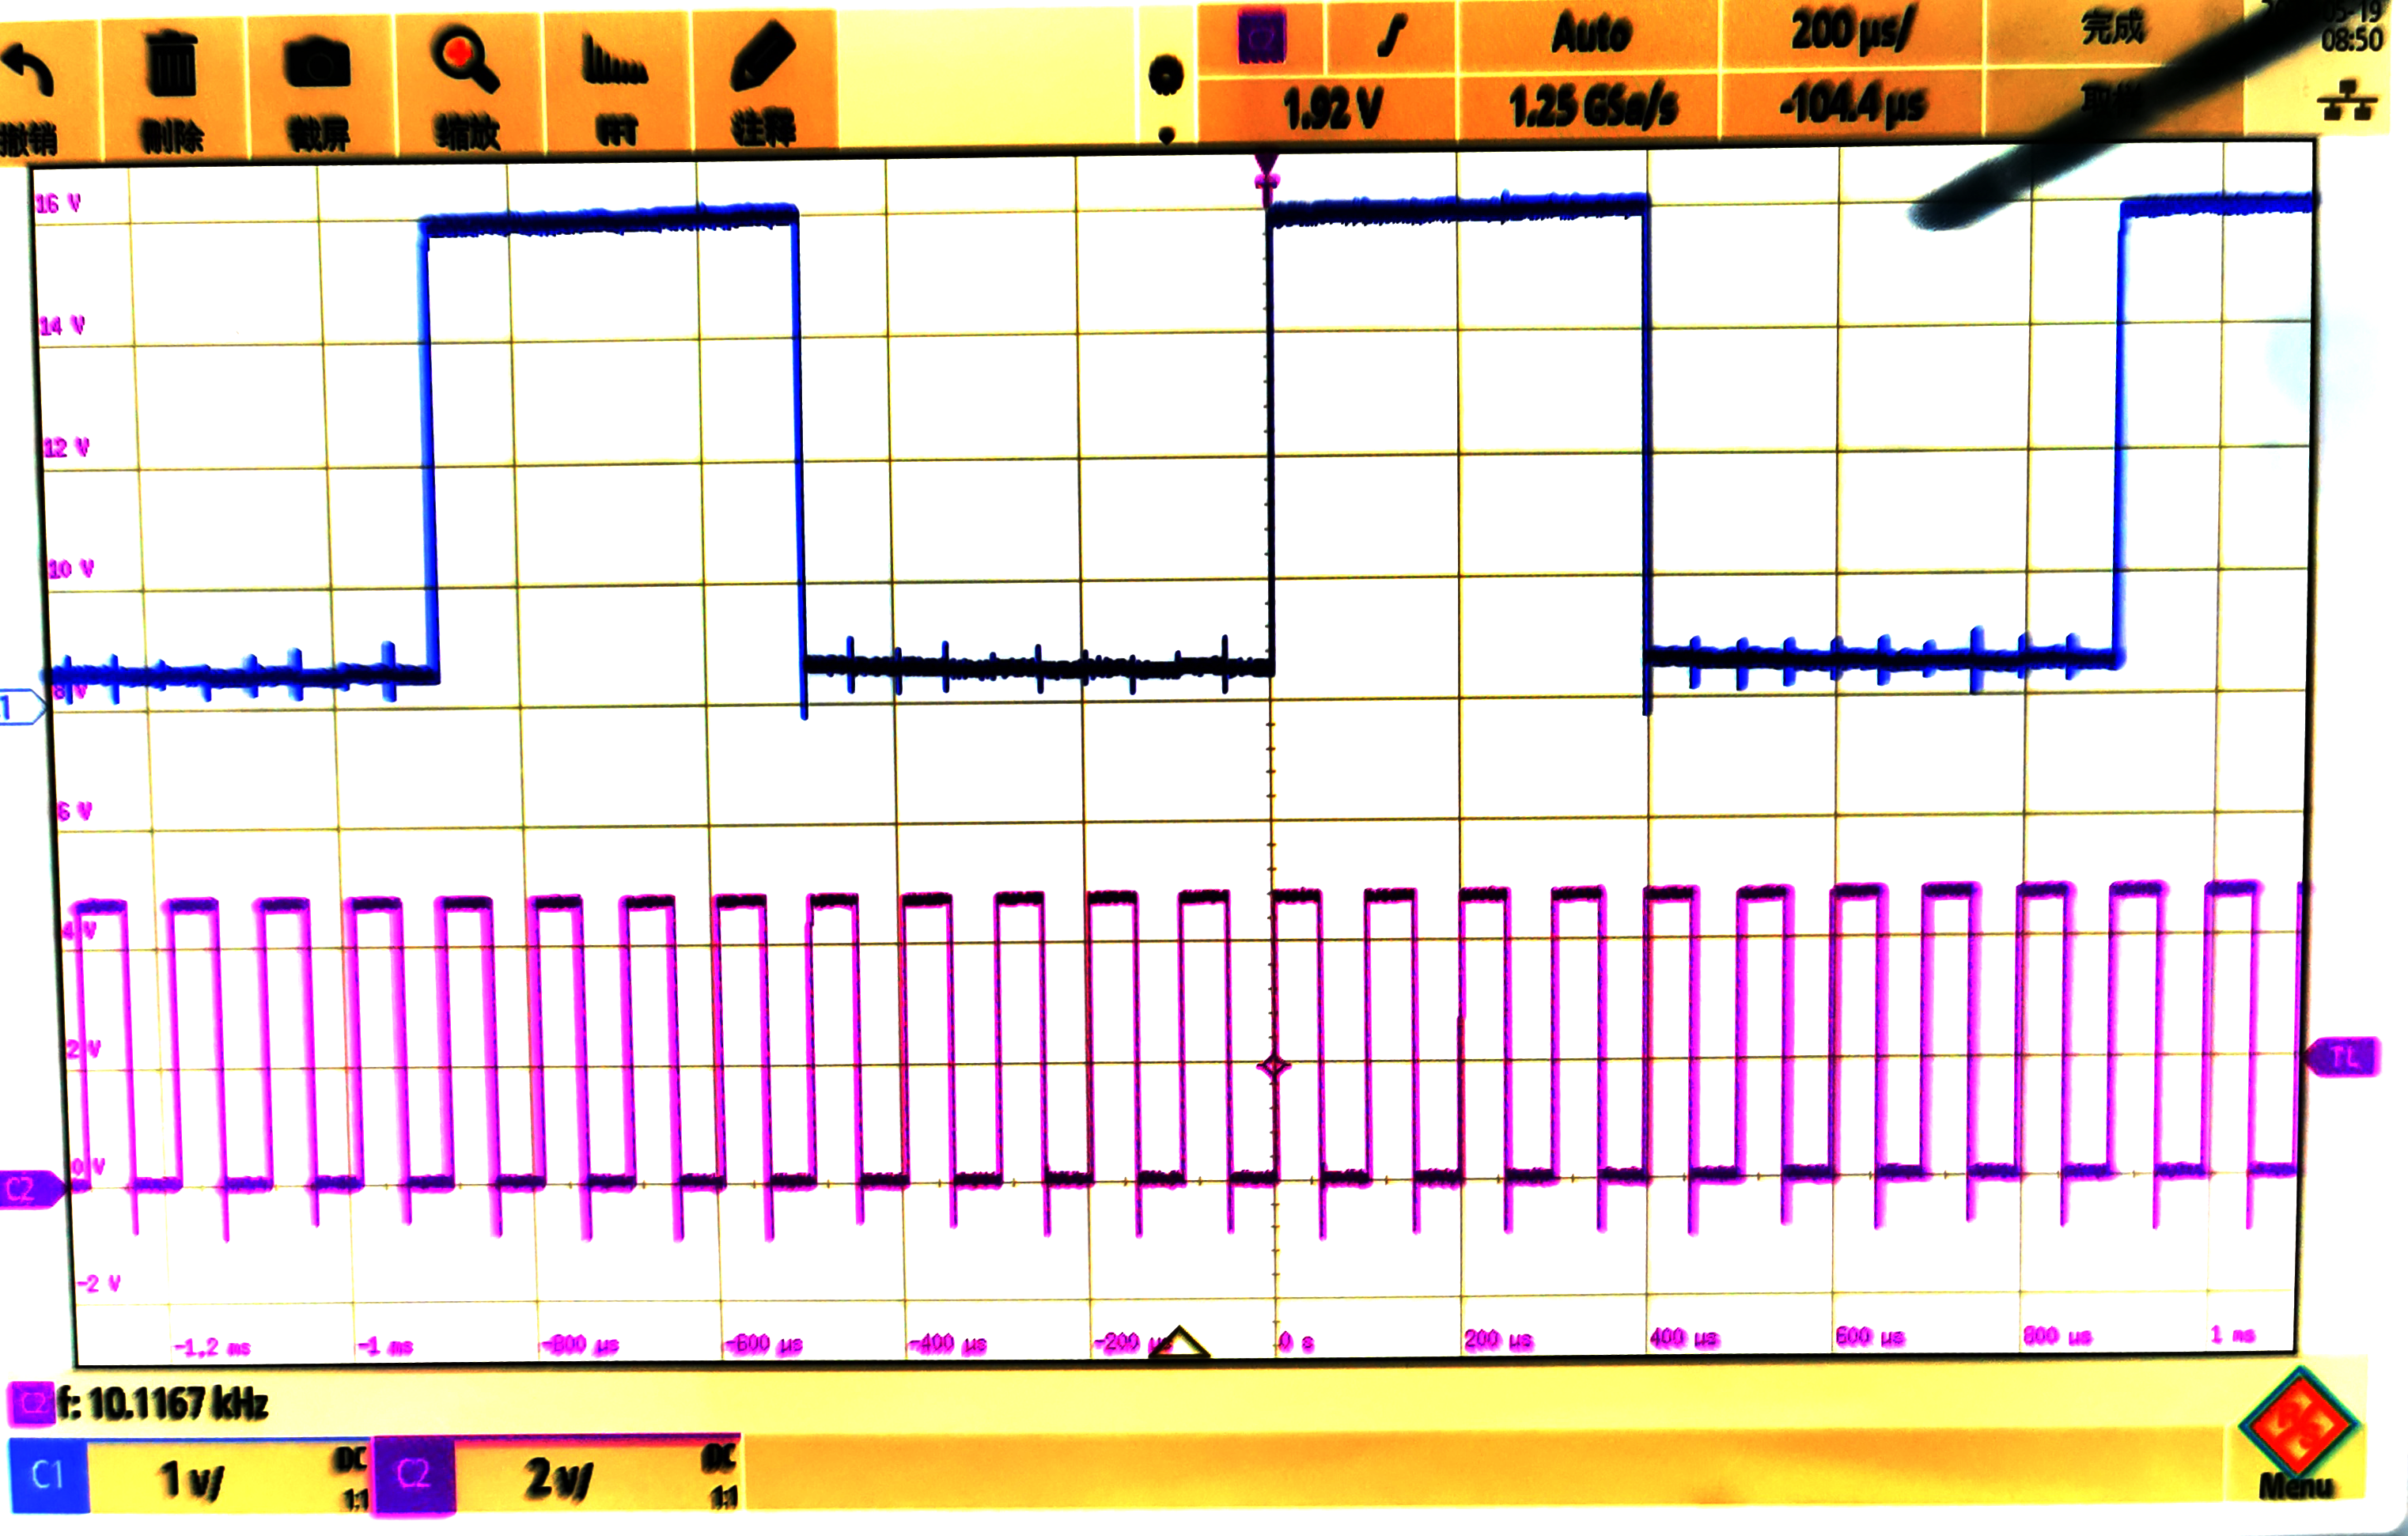
\includegraphics[width=3.5in]{H:/电子技术试验/4-21/9-q2.png}   
    \caption{$CLK/Q2$}   
    \label{fig:side:a}   
  \end{minipage}%   
  \begin{minipage}[t]{0.5\linewidth}   
    \centering   
    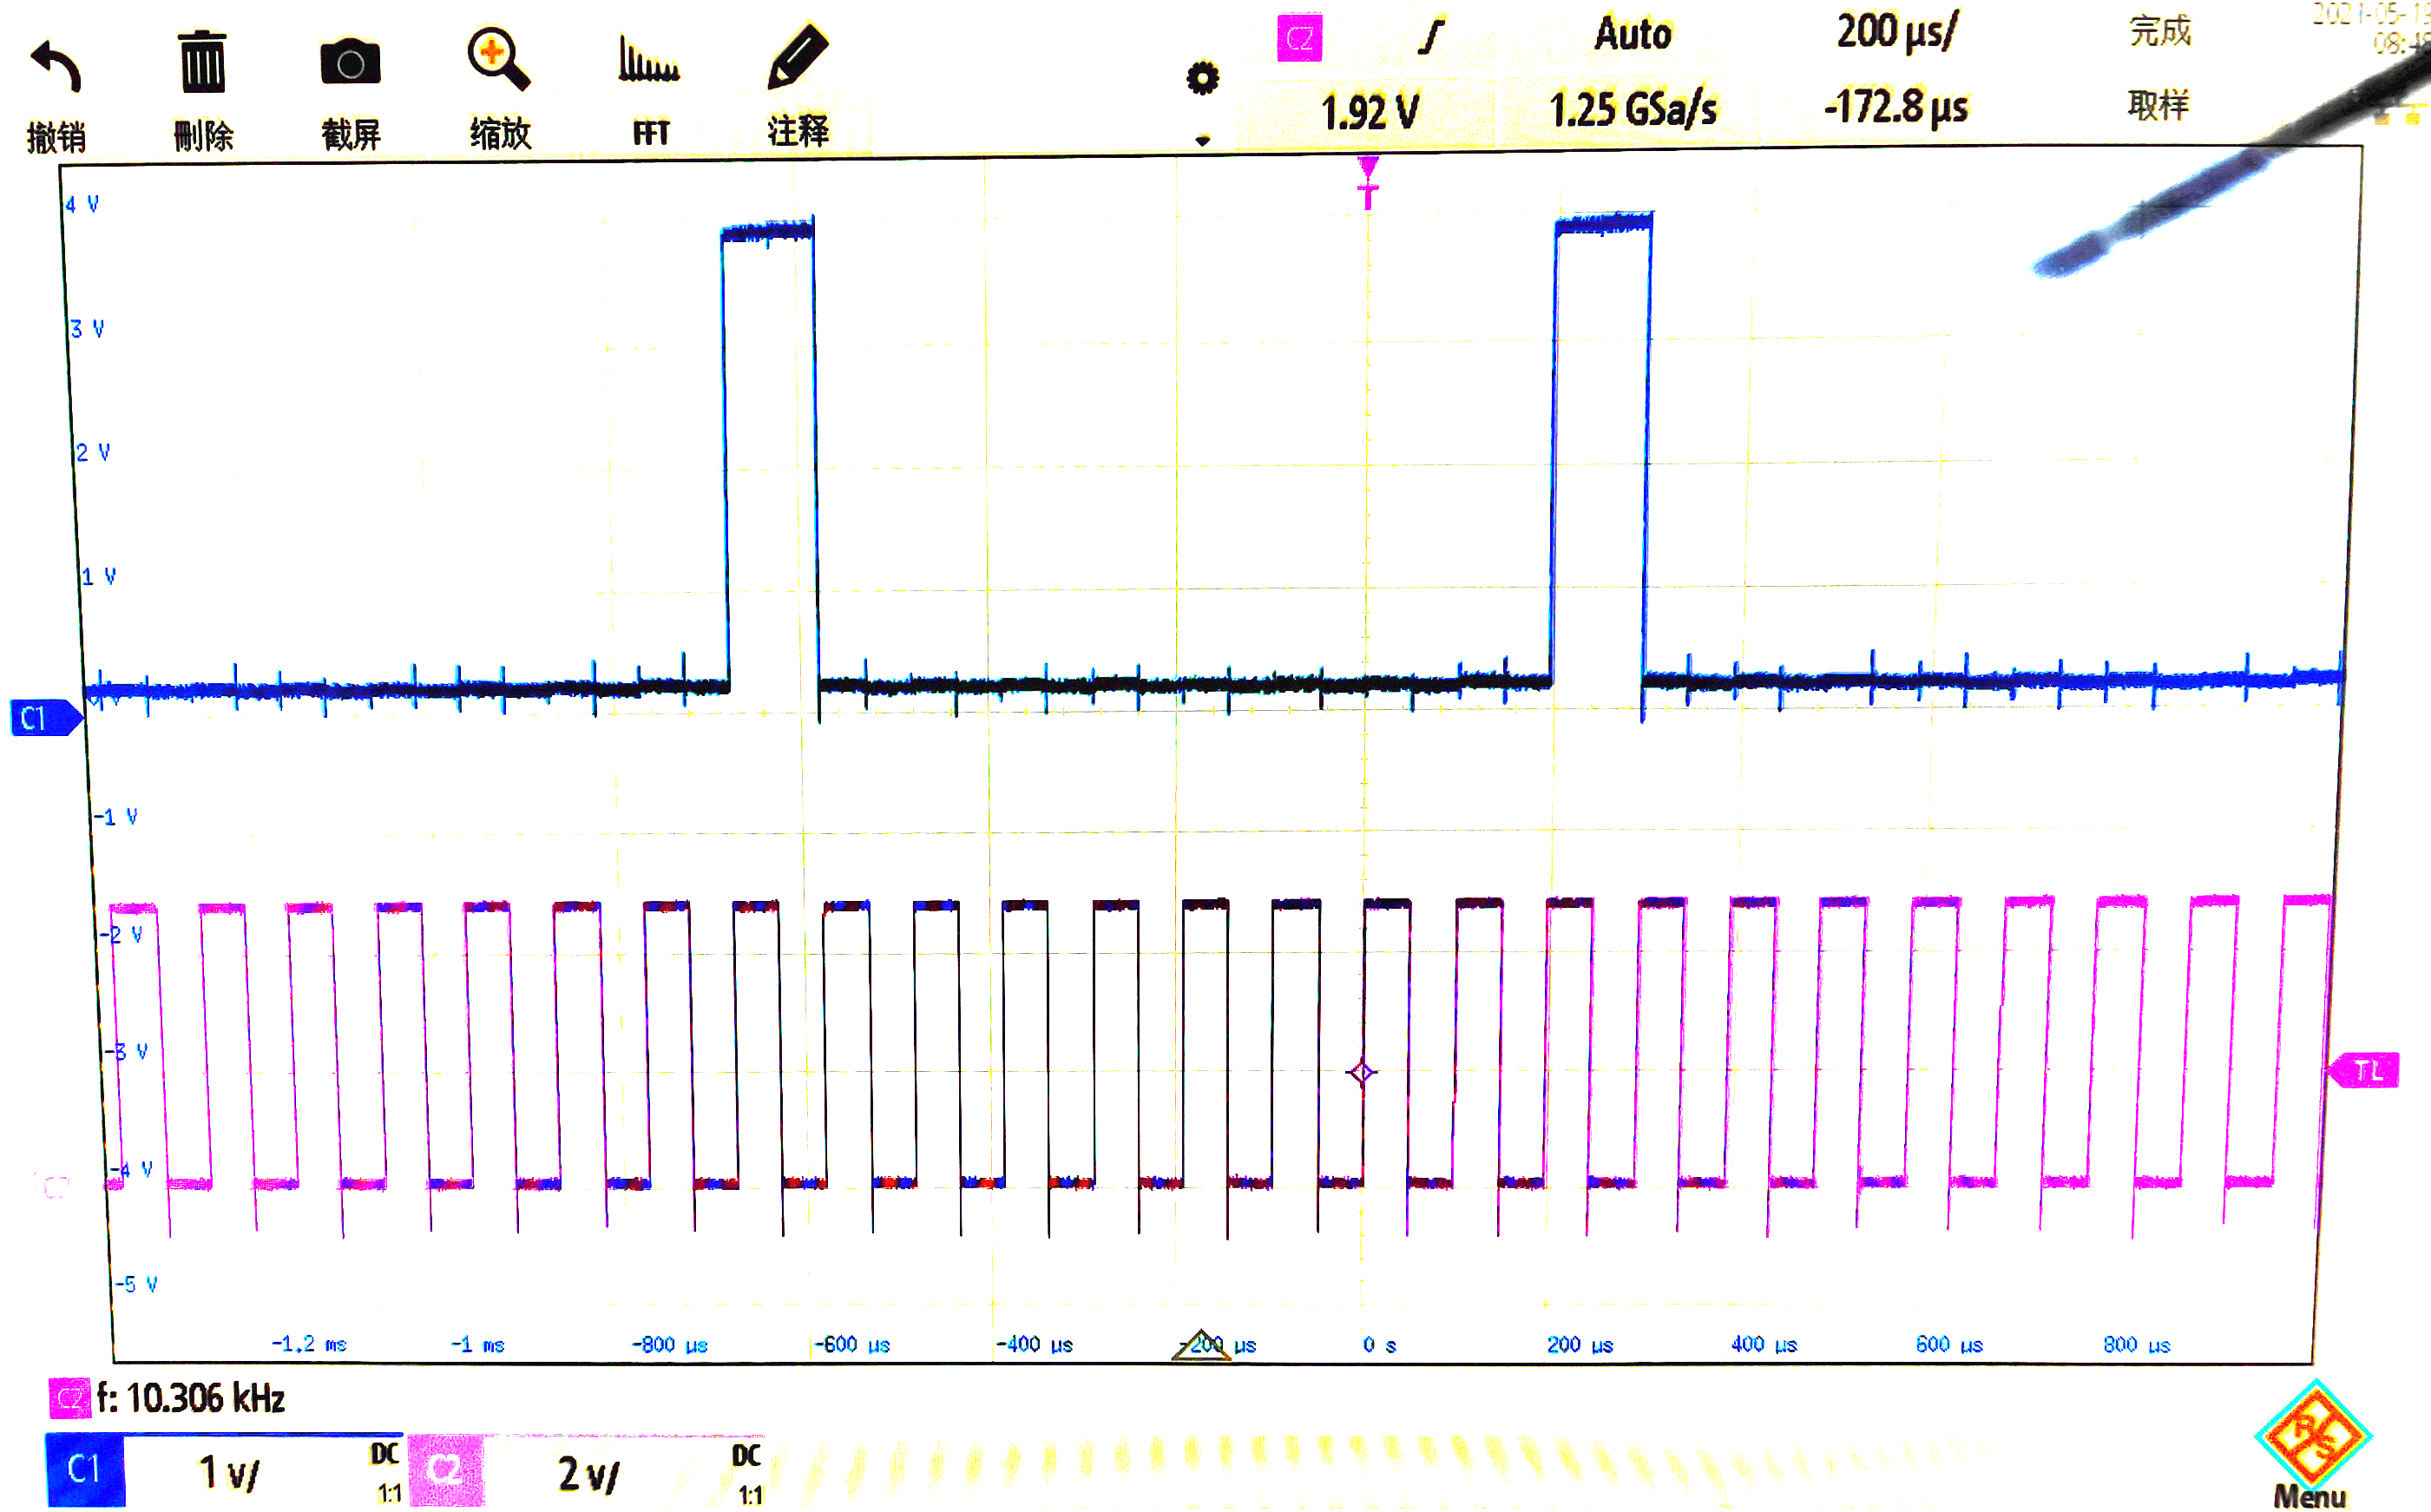
\includegraphics[width=3.5in]{H:/电子技术试验/4-21/9-q3.png}   
    \caption{$CLK/Q3$}   
    \label{fig:side:b}   
  \end{minipage}   
\end{figure}


\section{结论}

74LS161的性质符合预期\par
9分频器和12分频器的输出结果符合预期\par

\end{document}